% Options for packages loaded elsewhere
\PassOptionsToPackage{unicode}{hyperref}
\PassOptionsToPackage{hyphens}{url}
%
\documentclass[
]{article}
\usepackage{lmodern}
\usepackage{amssymb,amsmath}
\usepackage{ifxetex,ifluatex}
\ifnum 0\ifxetex 1\fi\ifluatex 1\fi=0 % if pdftex
  \usepackage[T1]{fontenc}
  \usepackage[utf8]{inputenc}
  \usepackage{textcomp} % provide euro and other symbols
\else % if luatex or xetex
  \usepackage{unicode-math}
  \defaultfontfeatures{Scale=MatchLowercase}
  \defaultfontfeatures[\rmfamily]{Ligatures=TeX,Scale=1}
\fi
% Use upquote if available, for straight quotes in verbatim environments
\IfFileExists{upquote.sty}{\usepackage{upquote}}{}
\IfFileExists{microtype.sty}{% use microtype if available
  \usepackage[]{microtype}
  \UseMicrotypeSet[protrusion]{basicmath} % disable protrusion for tt fonts
}{}
\makeatletter
\@ifundefined{KOMAClassName}{% if non-KOMA class
  \IfFileExists{parskip.sty}{%
    \usepackage{parskip}
  }{% else
    \setlength{\parindent}{0pt}
    \setlength{\parskip}{6pt plus 2pt minus 1pt}}
}{% if KOMA class
  \KOMAoptions{parskip=half}}
\makeatother
\usepackage{xcolor}
\IfFileExists{xurl.sty}{\usepackage{xurl}}{} % add URL line breaks if available
\IfFileExists{bookmark.sty}{\usepackage{bookmark}}{\usepackage{hyperref}}
\hypersetup{
  pdftitle={Datos Omicos PEC2},
  pdfauthor={Eva Mª Ruiz Macias},
  hidelinks,
  pdfcreator={LaTeX via pandoc}}
\urlstyle{same} % disable monospaced font for URLs
\usepackage[margin=1in]{geometry}
\usepackage{color}
\usepackage{fancyvrb}
\newcommand{\VerbBar}{|}
\newcommand{\VERB}{\Verb[commandchars=\\\{\}]}
\DefineVerbatimEnvironment{Highlighting}{Verbatim}{commandchars=\\\{\}}
% Add ',fontsize=\small' for more characters per line
\usepackage{framed}
\definecolor{shadecolor}{RGB}{248,248,248}
\newenvironment{Shaded}{\begin{snugshade}}{\end{snugshade}}
\newcommand{\AlertTok}[1]{\textcolor[rgb]{0.94,0.16,0.16}{#1}}
\newcommand{\AnnotationTok}[1]{\textcolor[rgb]{0.56,0.35,0.01}{\textbf{\textit{#1}}}}
\newcommand{\AttributeTok}[1]{\textcolor[rgb]{0.77,0.63,0.00}{#1}}
\newcommand{\BaseNTok}[1]{\textcolor[rgb]{0.00,0.00,0.81}{#1}}
\newcommand{\BuiltInTok}[1]{#1}
\newcommand{\CharTok}[1]{\textcolor[rgb]{0.31,0.60,0.02}{#1}}
\newcommand{\CommentTok}[1]{\textcolor[rgb]{0.56,0.35,0.01}{\textit{#1}}}
\newcommand{\CommentVarTok}[1]{\textcolor[rgb]{0.56,0.35,0.01}{\textbf{\textit{#1}}}}
\newcommand{\ConstantTok}[1]{\textcolor[rgb]{0.00,0.00,0.00}{#1}}
\newcommand{\ControlFlowTok}[1]{\textcolor[rgb]{0.13,0.29,0.53}{\textbf{#1}}}
\newcommand{\DataTypeTok}[1]{\textcolor[rgb]{0.13,0.29,0.53}{#1}}
\newcommand{\DecValTok}[1]{\textcolor[rgb]{0.00,0.00,0.81}{#1}}
\newcommand{\DocumentationTok}[1]{\textcolor[rgb]{0.56,0.35,0.01}{\textbf{\textit{#1}}}}
\newcommand{\ErrorTok}[1]{\textcolor[rgb]{0.64,0.00,0.00}{\textbf{#1}}}
\newcommand{\ExtensionTok}[1]{#1}
\newcommand{\FloatTok}[1]{\textcolor[rgb]{0.00,0.00,0.81}{#1}}
\newcommand{\FunctionTok}[1]{\textcolor[rgb]{0.00,0.00,0.00}{#1}}
\newcommand{\ImportTok}[1]{#1}
\newcommand{\InformationTok}[1]{\textcolor[rgb]{0.56,0.35,0.01}{\textbf{\textit{#1}}}}
\newcommand{\KeywordTok}[1]{\textcolor[rgb]{0.13,0.29,0.53}{\textbf{#1}}}
\newcommand{\NormalTok}[1]{#1}
\newcommand{\OperatorTok}[1]{\textcolor[rgb]{0.81,0.36,0.00}{\textbf{#1}}}
\newcommand{\OtherTok}[1]{\textcolor[rgb]{0.56,0.35,0.01}{#1}}
\newcommand{\PreprocessorTok}[1]{\textcolor[rgb]{0.56,0.35,0.01}{\textit{#1}}}
\newcommand{\RegionMarkerTok}[1]{#1}
\newcommand{\SpecialCharTok}[1]{\textcolor[rgb]{0.00,0.00,0.00}{#1}}
\newcommand{\SpecialStringTok}[1]{\textcolor[rgb]{0.31,0.60,0.02}{#1}}
\newcommand{\StringTok}[1]{\textcolor[rgb]{0.31,0.60,0.02}{#1}}
\newcommand{\VariableTok}[1]{\textcolor[rgb]{0.00,0.00,0.00}{#1}}
\newcommand{\VerbatimStringTok}[1]{\textcolor[rgb]{0.31,0.60,0.02}{#1}}
\newcommand{\WarningTok}[1]{\textcolor[rgb]{0.56,0.35,0.01}{\textbf{\textit{#1}}}}
\usepackage{graphicx,grffile}
\makeatletter
\def\maxwidth{\ifdim\Gin@nat@width>\linewidth\linewidth\else\Gin@nat@width\fi}
\def\maxheight{\ifdim\Gin@nat@height>\textheight\textheight\else\Gin@nat@height\fi}
\makeatother
% Scale images if necessary, so that they will not overflow the page
% margins by default, and it is still possible to overwrite the defaults
% using explicit options in \includegraphics[width, height, ...]{}
\setkeys{Gin}{width=\maxwidth,height=\maxheight,keepaspectratio}
% Set default figure placement to htbp
\makeatletter
\def\fps@figure{htbp}
\makeatother
\setlength{\emergencystretch}{3em} % prevent overfull lines
\providecommand{\tightlist}{%
  \setlength{\itemsep}{0pt}\setlength{\parskip}{0pt}}
\setcounter{secnumdepth}{-\maxdimen} % remove section numbering
\usepackage{booktabs}
\usepackage{longtable}
\usepackage{array}
\usepackage{multirow}
\usepackage{wrapfig}
\usepackage{float}
\usepackage{colortbl}
\usepackage{pdflscape}
\usepackage{tabu}
\usepackage{threeparttable}
\usepackage{threeparttablex}
\usepackage[normalem]{ulem}
\usepackage{makecell}
\usepackage{xcolor}

\title{Datos Omicos PEC2}
\author{Eva Mª Ruiz Macias}
\date{6 de junio, 2020}

\begin{document}
\maketitle

{
\setcounter{tocdepth}{2}
\tableofcontents
}
\hypertarget{introduccion}{%
\section{Introduccion}\label{introduccion}}

En este trabajo veremos como analizar los datos de conteo de RNA-seq
usando el paquete R, y más concretamente edgeR. Los puntos que se
tocaran van desde la lectura de los datos en R, hasta el control de
calidad, la realización de análisis de expresión diferencial y pruebas
de conjuntos de genes.

Los resultados de este trabajo se pueden encontrar en:

\url{https://github.com/Tortufuriaperru/PEC2DatosOmicos.git}

\hypertarget{objetivos}{%
\section{Objetivos}\label{objetivos}}

Se analizaran los datos de expresion de tejido tiroideo de diferentes
tipos: sin infiltración linfoidea, con pequeñas infiltraciones focales,
y con infiltración linfoide extensa siguiendo los pasos mencionados
anteriormente.

\hypertarget{materiales-y-muxe9todos}{%
\section{Materiales y métodos}\label{materiales-y-muxe9todos}}

\hypertarget{naturaleza-de-los-datos}{%
\subsection{Naturaleza de los datos}\label{naturaleza-de-los-datos}}

Para este trabajo contamos con dos archivos de datos llamados targets y
counts que contienen la información de las muestras de un estudio
obtenido del repositorio GTEx.

Dicho repositorio contiene datos de múltiples tipos en un total de 54
tejidos. En este trabajo utilizaremos los datos de expresión (RNA-seq)
pertenecientes a un análisis del tiroides, en donde se compararan tres
tipos de infiltración.

\hypertarget{metodos-para-el-analisis}{%
\subsection{Metodos para el analisis}\label{metodos-para-el-analisis}}

\hypertarget{identificaciuxf3n-de-grupos-y-quien-pertenece-a-cada-muestra.}{%
\subsubsection{Identificación de grupos y quien pertenece a cada
muestra.}\label{identificaciuxf3n-de-grupos-y-quien-pertenece-a-cada-muestra.}}

En el archivo original contamos con 292 muestras de los siguientes tipos

\begin{itemize}
\tightlist
\item
  Not infiltrated tissues (NIT): 236 samples
\item
  Small focal infiltrates (SFI): 42 samples
\item
  Extensive lymphoid infiltrates (ELI): 14 samples.
\end{itemize}

Nos quedaremos con 10 muestras de cada grupo, que se mostraran
posteriormente.

\hypertarget{lectura-de-datos-y-selecciuxf3n-de-muestra}{%
\subsubsection{Lectura de datos y selección de
muestra}\label{lectura-de-datos-y-selecciuxf3n-de-muestra}}

Procedemos a leer los archivos facilitados, y a seleccionar 10 muestras
de cada tipo (30 en total):

\begin{Shaded}
\begin{Highlighting}[]
\NormalTok{targets <-}\StringTok{  }\KeywordTok{read.csv}\NormalTok{(}\StringTok{"C:/PEC2DatosOmicos/data/targets.csv"}\NormalTok{, }\DataTypeTok{header =} \OtherTok{TRUE}\NormalTok{)}
\NormalTok{counts <-}\StringTok{  }\KeywordTok{read.csv2}\NormalTok{(}\StringTok{"C:/PEC2DatosOmicos/data/counts.csv"}\NormalTok{, }\DataTypeTok{header =} \OtherTok{TRUE}\NormalTok{, }\DataTypeTok{sep =} \StringTok{";"}\NormalTok{)}
\end{Highlighting}
\end{Shaded}

Seleccionamos la muestra de la siguiente forma:

\begin{Shaded}
\begin{Highlighting}[]
\KeywordTok{set.seed}\NormalTok{(}\DecValTok{321}\NormalTok{, }\DataTypeTok{sample.kind =} \StringTok{"Rounding"}\NormalTok{)}
\end{Highlighting}
\end{Shaded}

\begin{verbatim}
## Warning in set.seed(321, sample.kind = "Rounding"): non-uniform 'Rounding'
## sampler used
\end{verbatim}

\begin{Shaded}
\begin{Highlighting}[]
\CommentTok{# muestras de tamaño 10 por grupo}

\NormalTok{targetsample <-}\StringTok{ }\NormalTok{targets}\OperatorTok\KeywordTok{group_by}\NormalTok{(Group)}\OperatorTok\KeywordTok{sample_n}\NormalTok{(}\DataTypeTok{size =} \DecValTok{10}\NormalTok{, }\DataTypeTok{replace=}\NormalTok{F)}

\CommentTok{# desactivo el paquete para que no me de problemas despues}

\KeywordTok{detach}\NormalTok{(}\StringTok{"package:dplyr"}\NormalTok{, }\DataTypeTok{unload =} \OtherTok{TRUE}\NormalTok{)}
\end{Highlighting}
\end{Shaded}

\begin{verbatim}
## Warning: 'dplyr' namespace cannot be unloaded:
##   namespace 'dplyr' is imported by 'BiocFileCache', 'dbplyr' so cannot be unloaded
\end{verbatim}

\begin{Shaded}
\begin{Highlighting}[]
\CommentTok{# nos quedamos con los elementos seleccionados}

\NormalTok{seleccion <-}\StringTok{ }\KeywordTok{c}\NormalTok{(targetsample}\OperatorTok{$}\NormalTok{Sample_Name)}

\CommentTok{# ahora nos quedamos con los elementos que ocupan la misma posicion en el}
\CommentTok{# archivo counts quitando la variable X}
\NormalTok{selectcounts <-}\StringTok{ }\NormalTok{counts[}\DecValTok{2}\OperatorTok{:}\DecValTok{293}\NormalTok{][seleccion]}
\NormalTok{selectcounts <-}\StringTok{ }\KeywordTok{subset}\NormalTok{(counts[}\DecValTok{2}\OperatorTok{:}\DecValTok{293}\NormalTok{], }\DataTypeTok{select=}\NormalTok{seleccion)}
\CommentTok{# pasamos los nombres de los genes de la variable X a los nombres de las filas}
\KeywordTok{rownames}\NormalTok{(selectcounts) <-}\StringTok{ }\NormalTok{counts}\OperatorTok{$}\NormalTok{X}
\CommentTok{# quitamos los puntos de los nombres de las columnas para su tratamiento}
\CommentTok{# posterior}

\KeywordTok{rownames}\NormalTok{(selectcounts) <-}\StringTok{ }\KeywordTok{gsub}\NormalTok{(}\StringTok{"}\CharTok{\textbackslash{}\textbackslash{}}\StringTok{..*"}\NormalTok{, }\StringTok{""}\NormalTok{, }\KeywordTok{rownames}\NormalTok{(selectcounts),}
                                \DataTypeTok{fixed =} \OtherTok{FALSE}\NormalTok{)}
\KeywordTok{head}\NormalTok{(}\KeywordTok{rownames}\NormalTok{(selectcounts))}
\end{Highlighting}
\end{Shaded}

\begin{verbatim}
## [1] "ENSG00000223972" "ENSG00000227232" "ENSG00000243485" "ENSG00000237613"
## [5] "ENSG00000268020" "ENSG00000240361"
\end{verbatim}

\begin{Shaded}
\begin{Highlighting}[]
\NormalTok{grupos <-}\StringTok{ }\KeywordTok{rep}\NormalTok{(}\KeywordTok{c}\NormalTok{(}\StringTok{"ELI"}\NormalTok{, }\StringTok{"NIT"}\NormalTok{, }\StringTok{"SFI"}\NormalTok{), }\DataTypeTok{each=}\DecValTok{10}\NormalTok{)}

\CommentTok{#head(selectcounts,3)}
\KeywordTok{dim}\NormalTok{(selectcounts)}
\end{Highlighting}
\end{Shaded}

\begin{verbatim}
## [1] 56202    30
\end{verbatim}

\hypertarget{instalaciuxf3n-de-paquetes-r}{%
\subsubsection{Instalación de paquetes
R}\label{instalaciuxf3n-de-paquetes-r}}

El analisis se ha hecho utilizando el programa R y los paquetes
necesarios para dicho analisis son los siguientes:

require(knitr)

require(kableExtra)

require(ggplot2)

require(gplots)

require(limma)

require(Glimma)

require(edgeR)

require(stringr)

require(DESeq)

require(DESeq2)

require(RColorBrewer)

require(org.Hs.eg.db)

require(goseq)

require(GO.db)

require(dplyr)

\hypertarget{formato-de-los-datos}{%
\subsubsection{Formato de los datos}\label{formato-de-los-datos}}

edgeR funciona con tablas de recuentos de lecturas de enteros, donde las
filas correspondien a genes y las columnas a muestras independientes.

Se almacenaran los datos en un objeto de datos basado en listas llamado
DGEList.

Este tipo de objeto es fácil de usar porque puede manipularse como
cualquier lista en R.

\begin{Shaded}
\begin{Highlighting}[]
\NormalTok{grupos <-}\StringTok{ }\KeywordTok{rep}\NormalTok{(}\KeywordTok{c}\NormalTok{(}\StringTok{"ELI"}\NormalTok{, }\StringTok{"NIT"}\NormalTok{, }\StringTok{"SFI"}\NormalTok{), }\DataTypeTok{each=}\DecValTok{10}\NormalTok{)}
\CommentTok{# Creamos el objeto dGEList}
\NormalTok{dgList <-}\StringTok{ }\KeywordTok{DGEList}\NormalTok{(selectcounts, }\DataTypeTok{group=}\NormalTok{grupos)}
\CommentTok{# Mostramos los datos}
\KeywordTok{head}\NormalTok{(dgList, }\DecValTok{2}\NormalTok{)}
\end{Highlighting}
\end{Shaded}

\begin{verbatim}
## An object of class "DGEList"
## $counts
##                 GTEX.ZYY3.1926.SM.5GZXS GTEX.YJ89.0726.SM.5P9F7
## ENSG00000223972                       6                       4
## ENSG00000227232                    1003                    1325
##                 GTEX.11XUK.0226.SM.5EQLW GTEX.YFC4.2626.SM.5P9FQ
## ENSG00000223972                        0                       1
## ENSG00000227232                      419                    1472
##                 GTEX.13NZ9.1126.SM.5MR37 GTEX.R55G.0726.SM.2TC6J
## ENSG00000223972                        0                       3
## ENSG00000227232                     1002                     134
##                 GTEX.PLZ4.1226.SM.2I5FE GTEX.TMMY.0826.SM.33HB9
## ENSG00000223972                       5                       3
## ENSG00000227232                     489                     979
##                 GTEX.14AS3.0226.SM.5Q5B6 GTEX.13QJC.0826.SM.5RQKC
## ENSG00000223972                        0                        0
## ENSG00000227232                      834                      825
##                 GTEX.QV31.0726.SM.3GAEG GTEX.13OW7.0826.SM.5L3EL
## ENSG00000223972                       3                        0
## ENSG00000227232                     450                      629
##                 GTEX.X8HC.0726.SM.46MWG GTEX.11DXX.0226.SM.5P9HL
## ENSG00000223972                       0                        4
## ENSG00000227232                     879                      825
##                 GTEX.Q734.0526.SM.2I3EH GTEX.13113.0126.SM.5LZVX
## ENSG00000223972                       2                        1
## ENSG00000227232                     749                      687
##                 GTEX.R3RS.0726.SM.3GIJR GTEX.13S86.1126.SM.5RQJX
## ENSG00000223972                       1                        1
## ENSG00000227232                     176                      800
##                 GTEX.13FTY.0726.SM.5J2OH GTEX.ZYFC.0926.SM.5GZWW
## ENSG00000223972                        1                       1
## ENSG00000227232                      675                    1051
##                 GTEX.QLQ7.0726.SM.2I5G2 GTEX.ZLV1.0126.SM.4WWBZ
## ENSG00000223972                       6                       2
## ENSG00000227232                     666                     689
##                 GTEX.Y5V6.0526.SM.4VBRV GTEX.13FH7.0126.SM.5KLZ1
## ENSG00000223972                       3                        5
## ENSG00000227232                     482                      576
##                 GTEX.13NZ8.0226.SM.5J2OK GTEX.R55C.0626.SM.2TF4Q
## ENSG00000223972                        1                       9
## ENSG00000227232                     1164                     302
##                 GTEX.WYVS.0326.SM.3NM9V GTEX.131YS.0726.SM.5P9G9
## ENSG00000223972                       6                        1
## ENSG00000227232                     820                     1487
##                 GTEX.11GS4.0826.SM.5986J GTEX.13FXS.0726.SM.5LZXJ
## ENSG00000223972                        0                        5
## ENSG00000227232                      533                     1564
## 
## $samples
##                          group lib.size norm.factors
## GTEX.ZYY3.1926.SM.5GZXS    ELI 48915857            1
## GTEX.YJ89.0726.SM.5P9F7    ELI 73988083            1
## GTEX.11XUK.0226.SM.5EQLW   ELI 50019489            1
## GTEX.YFC4.2626.SM.5P9FQ    ELI 81226878            1
## GTEX.13NZ9.1126.SM.5MR37   ELI 61447691            1
## 25 more rows ...
\end{verbatim}

\begin{Shaded}
\begin{Highlighting}[]
\KeywordTok{names}\NormalTok{(dgList)}
\end{Highlighting}
\end{Shaded}

\begin{verbatim}
## [1] "counts"  "samples"
\end{verbatim}

\begin{Shaded}
\begin{Highlighting}[]
\NormalTok{dgList}\OperatorTok{$}\NormalTok{samples}
\end{Highlighting}
\end{Shaded}

\begin{verbatim}
##                          group lib.size norm.factors
## GTEX.ZYY3.1926.SM.5GZXS    ELI 48915857            1
## GTEX.YJ89.0726.SM.5P9F7    ELI 73988083            1
## GTEX.11XUK.0226.SM.5EQLW   ELI 50019489            1
## GTEX.YFC4.2626.SM.5P9FQ    ELI 81226878            1
## GTEX.13NZ9.1126.SM.5MR37   ELI 61447691            1
## GTEX.R55G.0726.SM.2TC6J    ELI 15483883            1
## GTEX.PLZ4.1226.SM.2I5FE    ELI 64441734            1
## GTEX.TMMY.0826.SM.33HB9    ELI 85633787            1
## GTEX.14AS3.0226.SM.5Q5B6   ELI 42011392            1
## GTEX.13QJC.0826.SM.5RQKC   ELI 48836801            1
## GTEX.QV31.0726.SM.3GAEG    NIT 49650895            1
## GTEX.13OW7.0826.SM.5L3EL   NIT 41666882            1
## GTEX.X8HC.0726.SM.46MWG    NIT 50137652            1
## GTEX.11DXX.0226.SM.5P9HL   NIT 85676907            1
## GTEX.Q734.0526.SM.2I3EH    NIT 50362382            1
## GTEX.13113.0126.SM.5LZVX   NIT 43630813            1
## GTEX.R3RS.0726.SM.3GIJR    NIT 12431887            1
## GTEX.13S86.1126.SM.5RQJX   NIT 40167105            1
## GTEX.13FTY.0726.SM.5J2OH   NIT 58965885            1
## GTEX.ZYFC.0926.SM.5GZWW    NIT 51417663            1
## GTEX.QLQ7.0726.SM.2I5G2    SFI 84712651            1
## GTEX.ZLV1.0126.SM.4WWBZ    SFI 55426907            1
## GTEX.Y5V6.0526.SM.4VBRV    SFI 68714782            1
## GTEX.13FH7.0126.SM.5KLZ1   SFI 66583792            1
## GTEX.13NZ8.0226.SM.5J2OK   SFI 59535746            1
## GTEX.R55C.0626.SM.2TF4Q    SFI 39862745            1
## GTEX.WYVS.0326.SM.3NM9V    SFI 76726397            1
## GTEX.131YS.0726.SM.5P9G9   SFI 67931798            1
## GTEX.11GS4.0826.SM.5986J   SFI 50383412            1
## GTEX.13FXS.0726.SM.5LZXJ   SFI 47570049            1
\end{verbatim}

\hypertarget{filtrado-para-eliminar-genes-poco-expresados}{%
\subsubsection{Filtrado para eliminar genes poco
expresados}\label{filtrado-para-eliminar-genes-poco-expresados}}

Los genes con recuentos muy bajos en todas las bibliotecas proporcionan
poca evidencia de expresión diferencial e interfieren con algunas de las
aproximaciones estadísticas que se utilizaran más adelante. También se
suman a la carga de las pruebas múltiples al estimar las tasas de
falsas, reduciendo el poder de detectar genes expresados
diferencialmente. Estos genes deben filtrarse antes de un análisis
posterior.

Hay algunas formas de filtrar los genes poco expresados. En este
conjunto de datos, elegimos retener genes si se expresan en un recuento
por millón (CPM) superior a 0,5 en al menos dos muestras.

Utilizaremos la función cpm de la biblioteca edgeR para generar los
valores de CPM y luego filtrarlos. Hay que tener en cuenta que al
convertir a CPM estamos normalizando las diferentes profundidades de
secuencia para cada muestra.

\begin{Shaded}
\begin{Highlighting}[]
\NormalTok{countsPerMillion <-}\StringTok{ }\KeywordTok{cpm}\NormalTok{(dgList)}
\KeywordTok{summary}\NormalTok{(countsPerMillion)}
\end{Highlighting}
\end{Shaded}

\begin{verbatim}
##  GTEX.ZYY3.1926.SM.5GZXS GTEX.YJ89.0726.SM.5P9F7 GTEX.11XUK.0226.SM.5EQLW
##  Min.   :    0.000       Min.   :    0.000       Min.   :    0.000       
##  1st Qu.:    0.000       1st Qu.:    0.000       1st Qu.:    0.000       
##  Median :    0.020       Median :    0.027       Median :    0.040       
##  Mean   :   17.793       Mean   :   17.793       Mean   :   17.793       
##  3rd Qu.:    3.128       3rd Qu.:    3.730       3rd Qu.:    3.459       
##  Max.   :27235.381       Max.   :24165.486       Max.   :21323.908       
##  GTEX.YFC4.2626.SM.5P9FQ GTEX.13NZ9.1126.SM.5MR37 GTEX.R55G.0726.SM.2TC6J
##  Min.   :    0.000       Min.   :    0.000        Min.   :    0.000      
##  1st Qu.:    0.000       1st Qu.:    0.000        1st Qu.:    0.000      
##  Median :    0.037       Median :    0.033        Median :    0.000      
##  Mean   :   17.793       Mean   :   17.793        Mean   :   17.793      
##  3rd Qu.:    4.050       3rd Qu.:    3.873        3rd Qu.:    3.746      
##  Max.   :12196.443       Max.   :10679.734        Max.   :24049.135      
##  GTEX.PLZ4.1226.SM.2I5FE GTEX.TMMY.0826.SM.33HB9 GTEX.14AS3.0226.SM.5Q5B6
##  Min.   :    0.000       Min.   :    0.00        Min.   :    0.00        
##  1st Qu.:    0.000       1st Qu.:    0.00        1st Qu.:    0.00        
##  Median :    0.031       Median :    0.04        Median :    0.05        
##  Mean   :   17.793       Mean   :   17.79        Mean   :   17.79        
##  3rd Qu.:    2.917       3rd Qu.:    2.80        3rd Qu.:    3.71        
##  Max.   :29715.308       Max.   :48667.11        Max.   :33592.56        
##  GTEX.13QJC.0826.SM.5RQKC GTEX.QV31.0726.SM.3GAEG GTEX.13OW7.0826.SM.5L3EL
##  Min.   :    0.000        Min.   :    0.00        Min.   :    0.000       
##  1st Qu.:    0.000        1st Qu.:    0.00        1st Qu.:    0.000       
##  Median :    0.041        Median :    0.02        Median :    0.024       
##  Mean   :   17.793        Mean   :   17.79        Mean   :   17.793       
##  3rd Qu.:    3.215        3rd Qu.:    2.26        3rd Qu.:    2.928       
##  Max.   :28440.253        Max.   :41245.10        Max.   :21764.816       
##  GTEX.X8HC.0726.SM.46MWG GTEX.11DXX.0226.SM.5P9HL GTEX.Q734.0526.SM.2I3EH
##  Min.   :    0.000       Min.   :    0.00         Min.   :    0.000      
##  1st Qu.:    0.000       1st Qu.:    0.00         1st Qu.:    0.000      
##  Median :    0.020       Median :    0.02         Median :    0.040      
##  Mean   :   17.793       Mean   :   17.79         Mean   :   17.793      
##  3rd Qu.:    2.847       3rd Qu.:    2.11         3rd Qu.:    3.058      
##  Max.   :13297.811       Max.   :36450.10         Max.   :24868.562      
##  GTEX.13113.0126.SM.5LZVX GTEX.R3RS.0726.SM.3GIJR GTEX.13S86.1126.SM.5RQJX
##  Min.   :    0.000        Min.   :    0.000       Min.   :    0.000       
##  1st Qu.:    0.000        1st Qu.:    0.000       1st Qu.:    0.000       
##  Median :    0.023        Median :    0.000       Median :    0.000       
##  Mean   :   17.793        Mean   :   17.793       Mean   :   17.793       
##  3rd Qu.:    2.842        3rd Qu.:    2.896       3rd Qu.:    2.415       
##  Max.   :27584.817        Max.   :28143.515       Max.   :29716.057       
##  GTEX.13FTY.0726.SM.5J2OH GTEX.ZYFC.0926.SM.5GZWW GTEX.QLQ7.0726.SM.2I5G2
##  Min.   :    0.000        Min.   :    0.00        Min.   :    0.00       
##  1st Qu.:    0.000        1st Qu.:    0.00        1st Qu.:    0.00       
##  Median :    0.034        Median :    0.02        Median :    0.02       
##  Mean   :   17.793        Mean   :   17.79        Mean   :   17.79       
##  3rd Qu.:    3.053        3rd Qu.:    2.65        3rd Qu.:    2.35       
##  Max.   :26554.744        Max.   :44670.33        Max.   :49250.75       
##  GTEX.ZLV1.0126.SM.4WWBZ GTEX.Y5V6.0526.SM.4VBRV GTEX.13FH7.0126.SM.5KLZ1
##  Min.   :    0.000       Min.   :    0.00        Min.   :    0.000       
##  1st Qu.:    0.000       1st Qu.:    0.00        1st Qu.:    0.000       
##  Median :    0.036       Median :    0.01        Median :    0.030       
##  Mean   :   17.793       Mean   :   17.79        Mean   :   17.793       
##  3rd Qu.:    3.248       3rd Qu.:    2.26        3rd Qu.:    2.628       
##  Max.   :19982.389       Max.   :49670.00        Max.   :31423.894       
##  GTEX.13NZ8.0226.SM.5J2OK GTEX.R55C.0626.SM.2TF4Q GTEX.WYVS.0326.SM.3NM9V
##  Min.   :    0.000        Min.   :    0.000       Min.   :    0.000      
##  1st Qu.:    0.000        1st Qu.:    0.000       1st Qu.:    0.000      
##  Median :    0.017        Median :    0.025       Median :    0.026      
##  Mean   :   17.793        Mean   :   17.793       Mean   :   17.793      
##  3rd Qu.:    2.839        3rd Qu.:    2.659       3rd Qu.:    3.089      
##  Max.   :13038.251        Max.   :31177.532       Max.   :28452.659      
##  GTEX.131YS.0726.SM.5P9G9 GTEX.11GS4.0826.SM.5986J GTEX.13FXS.0726.SM.5LZXJ
##  Min.   :    0.00         Min.   :    0.00         Min.   :    0.000       
##  1st Qu.:    0.00         1st Qu.:    0.00         1st Qu.:    0.000       
##  Median :    0.03         Median :    0.04         Median :    0.021       
##  Mean   :   17.79         Mean   :   17.79         Mean   :   17.793       
##  3rd Qu.:    3.47         3rd Qu.:    2.64         3rd Qu.:    3.195       
##  Max.   :34335.82         Max.   :31870.83         Max.   :18527.267
\end{verbatim}

\begin{Shaded}
\begin{Highlighting}[]
\CommentTok{# valores mayores que 0.5}
\NormalTok{countCheck <-}\StringTok{ }\NormalTok{countsPerMillion }\OperatorTok{>}\StringTok{ }\FloatTok{0.5}
\CommentTok{# Esto produce una salida con valores logicos TRUEs y FALSEs}
\KeywordTok{head}\NormalTok{(countCheck, }\DecValTok{2}\NormalTok{)}
\end{Highlighting}
\end{Shaded}

\begin{verbatim}
##                 GTEX.ZYY3.1926.SM.5GZXS GTEX.YJ89.0726.SM.5P9F7
## ENSG00000223972                   FALSE                   FALSE
## ENSG00000227232                    TRUE                    TRUE
##                 GTEX.11XUK.0226.SM.5EQLW GTEX.YFC4.2626.SM.5P9FQ
## ENSG00000223972                    FALSE                   FALSE
## ENSG00000227232                     TRUE                    TRUE
##                 GTEX.13NZ9.1126.SM.5MR37 GTEX.R55G.0726.SM.2TC6J
## ENSG00000223972                    FALSE                   FALSE
## ENSG00000227232                     TRUE                    TRUE
##                 GTEX.PLZ4.1226.SM.2I5FE GTEX.TMMY.0826.SM.33HB9
## ENSG00000223972                   FALSE                   FALSE
## ENSG00000227232                    TRUE                    TRUE
##                 GTEX.14AS3.0226.SM.5Q5B6 GTEX.13QJC.0826.SM.5RQKC
## ENSG00000223972                    FALSE                    FALSE
## ENSG00000227232                     TRUE                     TRUE
##                 GTEX.QV31.0726.SM.3GAEG GTEX.13OW7.0826.SM.5L3EL
## ENSG00000223972                   FALSE                    FALSE
## ENSG00000227232                    TRUE                     TRUE
##                 GTEX.X8HC.0726.SM.46MWG GTEX.11DXX.0226.SM.5P9HL
## ENSG00000223972                   FALSE                    FALSE
## ENSG00000227232                    TRUE                     TRUE
##                 GTEX.Q734.0526.SM.2I3EH GTEX.13113.0126.SM.5LZVX
## ENSG00000223972                   FALSE                    FALSE
## ENSG00000227232                    TRUE                     TRUE
##                 GTEX.R3RS.0726.SM.3GIJR GTEX.13S86.1126.SM.5RQJX
## ENSG00000223972                   FALSE                    FALSE
## ENSG00000227232                    TRUE                     TRUE
##                 GTEX.13FTY.0726.SM.5J2OH GTEX.ZYFC.0926.SM.5GZWW
## ENSG00000223972                    FALSE                   FALSE
## ENSG00000227232                     TRUE                    TRUE
##                 GTEX.QLQ7.0726.SM.2I5G2 GTEX.ZLV1.0126.SM.4WWBZ
## ENSG00000223972                   FALSE                   FALSE
## ENSG00000227232                    TRUE                    TRUE
##                 GTEX.Y5V6.0526.SM.4VBRV GTEX.13FH7.0126.SM.5KLZ1
## ENSG00000223972                   FALSE                    FALSE
## ENSG00000227232                    TRUE                     TRUE
##                 GTEX.13NZ8.0226.SM.5J2OK GTEX.R55C.0626.SM.2TF4Q
## ENSG00000223972                    FALSE                   FALSE
## ENSG00000227232                     TRUE                    TRUE
##                 GTEX.WYVS.0326.SM.3NM9V GTEX.131YS.0726.SM.5P9G9
## ENSG00000223972                   FALSE                    FALSE
## ENSG00000227232                    TRUE                     TRUE
##                 GTEX.11GS4.0826.SM.5986J GTEX.13FXS.0726.SM.5LZXJ
## ENSG00000223972                    FALSE                    FALSE
## ENSG00000227232                     TRUE                     TRUE
\end{verbatim}

\begin{Shaded}
\begin{Highlighting}[]
\CommentTok{# Cuantos trues hay en cada fila}
\KeywordTok{table}\NormalTok{(}\KeywordTok{rowSums}\NormalTok{(countCheck))}
\end{Highlighting}
\end{Shaded}

\begin{verbatim}
## 
##     0     1     2     3     4     5     6     7     8     9    10    11    12 
## 32941  1259   658   474   361   322   259   235   250   208   215   188   182 
##    13    14    15    16    17    18    19    20    21    22    23    24    25 
##   184   184   201   180   149   154   181   157   171   158   193   212   172 
##    26    27    28    29    30 
##   223   268   355   573 14935
\end{verbatim}

\begin{Shaded}
\begin{Highlighting}[]
\CommentTok{# Nos quedamos con los que tengan al menos 2 TRUES}
\NormalTok{keep <-}\StringTok{ }\KeywordTok{which}\NormalTok{(}\KeywordTok{rowSums}\NormalTok{(countCheck) }\OperatorTok{>=}\StringTok{ }\DecValTok{2}\NormalTok{)}
\NormalTok{dgList <-}\StringTok{ }\NormalTok{dgList[keep,]}
\KeywordTok{summary}\NormalTok{(}\KeywordTok{cpm}\NormalTok{(dgList))}
\end{Highlighting}
\end{Shaded}

\begin{verbatim}
##  GTEX.ZYY3.1926.SM.5GZXS GTEX.YJ89.0726.SM.5P9F7 GTEX.11XUK.0226.SM.5EQLW
##  Min.   :    0.000       Min.   :    0.000       Min.   :    0.00        
##  1st Qu.:    1.083       1st Qu.:    1.284       1st Qu.:    1.22        
##  Median :   10.610       Median :   11.867       Median :   11.02        
##  Mean   :   45.418       Mean   :   45.414       Mean   :   45.41        
##  3rd Qu.:   40.105       3rd Qu.:   43.575       3rd Qu.:   40.82        
##  Max.   :27235.381       Max.   :24165.486       Max.   :21323.91        
##  GTEX.YFC4.2626.SM.5P9FQ GTEX.13NZ9.1126.SM.5MR37 GTEX.R55G.0726.SM.2TC6J
##  Min.   :    0.000       Min.   :    0.000        Min.   :    0.000      
##  1st Qu.:    1.465       1st Qu.:    1.334        1st Qu.:    1.356      
##  Median :   12.453       Median :   12.352        Median :   11.560      
##  Mean   :   45.404       Mean   :   45.413        Mean   :   45.405      
##  3rd Qu.:   44.366       3rd Qu.:   46.295        3rd Qu.:   42.237      
##  Max.   :12196.443       Max.   :10679.734        Max.   :24049.135      
##  GTEX.PLZ4.1226.SM.2I5FE GTEX.TMMY.0826.SM.33HB9 GTEX.14AS3.0226.SM.5Q5B6
##  Min.   :    0.000       Min.   :    0.00        Min.   :    0.00        
##  1st Qu.:    1.013       1st Qu.:    0.97        1st Qu.:    1.29        
##  Median :    9.846       Median :    9.63        Median :   11.95        
##  Mean   :   45.415       Mean   :   45.41        Mean   :   45.41        
##  3rd Qu.:   40.657       3rd Qu.:   38.56        3rd Qu.:   43.13        
##  Max.   :29715.308       Max.   :48667.11        Max.   :33592.56        
##  GTEX.13QJC.0826.SM.5RQKC GTEX.QV31.0726.SM.3GAEG GTEX.13OW7.0826.SM.5L3EL
##  Min.   :    0.000        Min.   :    0.00        Min.   :    0.000       
##  1st Qu.:    1.126        1st Qu.:    0.79        1st Qu.:    1.038       
##  Median :   10.402        Median :    9.10        Median :   10.104       
##  Mean   :   45.415        Mean   :   45.42        Mean   :   45.413       
##  3rd Qu.:   40.584        3rd Qu.:   39.35        3rd Qu.:   41.376       
##  Max.   :28440.253        Max.   :41245.10        Max.   :21764.816       
##  GTEX.X8HC.0726.SM.46MWG GTEX.11DXX.0226.SM.5P9HL GTEX.Q734.0526.SM.2I3EH
##  Min.   :    0.000       Min.   :    0.00         Min.   :    0.000      
##  1st Qu.:    0.977       1st Qu.:    0.70         1st Qu.:    1.033      
##  Median :    9.733       Median :    8.53         Median :   10.831      
##  Mean   :   45.416       Mean   :   45.42         Mean   :   45.415      
##  3rd Qu.:   41.785       3rd Qu.:   38.41         3rd Qu.:   41.435      
##  Max.   :13297.811       Max.   :36450.10         Max.   :24868.562      
##  GTEX.13113.0126.SM.5LZVX GTEX.R3RS.0726.SM.3GIJR GTEX.13S86.1126.SM.5RQJX
##  Min.   :    0.000        Min.   :    0.000       Min.   :    0.000       
##  1st Qu.:    1.008        1st Qu.:    1.046       1st Qu.:    0.797       
##  Median :    9.901        Median :   10.055       Median :    9.460       
##  Mean   :   45.416        Mean   :   45.410       Mean   :   45.426       
##  3rd Qu.:   41.072        3rd Qu.:   40.541       3rd Qu.:   39.510       
##  Max.   :27584.817        Max.   :28143.515       Max.   :29716.057       
##  GTEX.13FTY.0726.SM.5J2OH GTEX.ZYFC.0926.SM.5GZWW GTEX.QLQ7.0726.SM.2I5G2
##  Min.   :    0.000        Min.   :    0.00        Min.   :    0.00       
##  1st Qu.:    1.034        1st Qu.:    0.91        1st Qu.:    0.81       
##  Median :   10.710        Median :    9.56        Median :    8.91       
##  Mean   :   45.417        Mean   :   45.42        Mean   :   45.42       
##  3rd Qu.:   41.834        3rd Qu.:   41.39        3rd Qu.:   39.07       
##  Max.   :26554.744        Max.   :44670.33        Max.   :49250.75       
##  GTEX.ZLV1.0126.SM.4WWBZ GTEX.Y5V6.0526.SM.4VBRV GTEX.13FH7.0126.SM.5KLZ1
##  Min.   :    0.000       Min.   :    0.00        Min.   :    0.000       
##  1st Qu.:    1.083       1st Qu.:    0.76        1st Qu.:    0.916       
##  Median :   11.240       Median :    8.95        Median :    9.529       
##  Mean   :   45.416       Mean   :   45.43        Mean   :   45.422       
##  3rd Qu.:   42.069       3rd Qu.:   39.42        3rd Qu.:   39.589       
##  Max.   :19982.389       Max.   :49670.00        Max.   :31423.894       
##  GTEX.13NZ8.0226.SM.5J2OK GTEX.R55C.0626.SM.2TF4Q GTEX.WYVS.0326.SM.3NM9V
##  Min.   :    0.000        Min.   :    0.000       Min.   :    0.000      
##  1st Qu.:    0.957        1st Qu.:    0.928       1st Qu.:    1.069      
##  Median :   10.221        Median :    9.708       Median :   10.518      
##  Mean   :   45.418        Mean   :   45.416       Mean   :   45.414      
##  3rd Qu.:   43.419        3rd Qu.:   41.267       3rd Qu.:   42.358      
##  Max.   :13038.251        Max.   :31177.532       Max.   :28452.659      
##  GTEX.131YS.0726.SM.5P9G9 GTEX.11GS4.0826.SM.5986J GTEX.13FXS.0726.SM.5LZXJ
##  Min.   :    0.00         Min.   :    0.00         Min.   :    0.000       
##  1st Qu.:    1.21         1st Qu.:    0.99         1st Qu.:    1.051       
##  Median :   10.94         Median :    9.23         Median :   11.173       
##  Mean   :   45.42         Mean   :   45.42         Mean   :   45.422       
##  3rd Qu.:   40.91         3rd Qu.:   39.79         3rd Qu.:   42.669       
##  Max.   :34335.82         Max.   :31870.83         Max.   :18527.267
\end{verbatim}

\begin{Shaded}
\begin{Highlighting}[]
\KeywordTok{dim}\NormalTok{(dgList)}
\end{Highlighting}
\end{Shaded}

\begin{verbatim}
## [1] 22002    30
\end{verbatim}

Esto reduce el conjunto de datos de 56202 genes a 22002. Para los genes
filtrados, hay muy poca potencia para detectar la expresión diferencial,
por lo que el filtrado pierde poca información.

\hypertarget{control-de-calidad}{%
\subsubsection{Control de calidad}\label{control-de-calidad}}

Una vez filtrados los genes con poca expresión y almacenados los datos
en el objeto que hemos creado, veamos la calidad de los datos.

Primero, podemos verificar cuántas lecturas tenemos para cada muestra:

\begin{Shaded}
\begin{Highlighting}[]
\NormalTok{dgList}\OperatorTok{$}\NormalTok{samples}\OperatorTok{$}\NormalTok{lib.size}
\end{Highlighting}
\end{Shaded}

\begin{verbatim}
##  [1] 48915857 73988083 50019489 81226878 61447691 15483883 64441734 85633787
##  [9] 42011392 48836801 49650895 41666882 50137652 85676907 50362382 43630813
## [17] 12431887 40167105 58965885 51417663 84712651 55426907 68714782 66583792
## [25] 59535746 39862745 76726397 67931798 50383412 47570049
\end{verbatim}

Hay que tener en cuenta que el ``size factor'' de DSeq no es igual que
``norm factor'' de edgeR.

También podemos trazar los tamaños de la biblioteca como un diagrama de
barras para ver si hay más discrepancias entre las muestras más
fácilmente

\begin{Shaded}
\begin{Highlighting}[]
\KeywordTok{barplot}\NormalTok{(dgList}\OperatorTok{$}\NormalTok{samples}\OperatorTok{$}\NormalTok{lib.size, }\DataTypeTok{names=}\KeywordTok{colnames}\NormalTok{(dgList), }\DataTypeTok{las=}\DecValTok{2}\NormalTok{)}
\KeywordTok{abline}\NormalTok{(}\DataTypeTok{h=}\FloatTok{20e6}\NormalTok{, }\DataTypeTok{lty=}\DecValTok{2}\NormalTok{)}
\end{Highlighting}
\end{Shaded}

\includegraphics{RuizMacias_EvaM_PEC2_ADO_files/figure-latex/unnamed-chunk-8-1.pdf}

Los datos de recuento no se distribuyen normalmente. Vamos a hacer
diagramas de cajas para verificar la distribución de los recuentos de
lectura en la escala log2. Podemos usar la funcion cpm para obtener
recuentos de log2 por millón, que se corrigen para los diferentes
tamaños de biblioteca. La funcion cpmf también agrega un pequeño
desplazamiento para evitar tomar el registro de cero.

\begin{Shaded}
\begin{Highlighting}[]
\KeywordTok{boxplot}\NormalTok{(}\KeywordTok{cpm}\NormalTok{(dgList, }\DataTypeTok{log =} \OtherTok{TRUE}\NormalTok{), }\DataTypeTok{xlab=}\StringTok{""}\NormalTok{, }\DataTypeTok{ylab=}\StringTok{"Log2 counts por millon"}\NormalTok{,}\DataTypeTok{las=}\DecValTok{2}\NormalTok{)}
\CommentTok{# Añadimos la mediana logCPM en color azul}
\KeywordTok{abline}\NormalTok{(}\DataTypeTok{h=}\KeywordTok{median}\NormalTok{(}\KeywordTok{cpm}\NormalTok{(dgList, }\DataTypeTok{log =} \OtherTok{TRUE}\NormalTok{)),}\DataTypeTok{col=}\StringTok{"blue"}\NormalTok{)}
\KeywordTok{title}\NormalTok{(}\StringTok{"Boxplots de logCPMs (sin normalizar)"}\NormalTok{)}
\end{Highlighting}
\end{Shaded}

\includegraphics{RuizMacias_EvaM_PEC2_ADO_files/figure-latex/unnamed-chunk-9-1.pdf}

De los diagramas de caja vemos que, en general, las distribuciones de
densidad de las intensidades logarítmicas en bruto no son idénticas pero
tampoco muy diferentes.

Un MDSplot es una visualización de un análisis de componentes
principales, que determina las mayores fuentes de variación en los
datos.Muestra distancias, en términos de coeficiente de variación
biológica (BCV), entre muestras.

Un análisis de componentes principales es un ejemplo de un análisis no
supervisado, donde no necesitamos especificar los grupos. Si el
experimento está bien controlado y ha funcionado bien, lo que esperamos
ver es que las mayores fuentes de variación en los datos son los grupos
en los que estamos interesados. También es una herramienta muy útil para
el control de calidad y la comprobación de valores atípicos. Podemos
usar la funcion plotMDS para crear el diagrama MDS.

\begin{Shaded}
\begin{Highlighting}[]
\KeywordTok{plotMDS}\NormalTok{(dgList, }\DataTypeTok{labels=}\NormalTok{dgList}\OperatorTok{$}\NormalTok{samples}\OperatorTok{$}\NormalTok{group,}
        \DataTypeTok{cex=}\FloatTok{0.75}\NormalTok{,}
        \DataTypeTok{xlim=}\KeywordTok{c}\NormalTok{(}\OperatorTok{-}\DecValTok{4}\NormalTok{, }\DecValTok{5}\NormalTok{),}
        \DataTypeTok{col=}\KeywordTok{as.numeric}\NormalTok{(dgList}\OperatorTok{$}\NormalTok{samples}\OperatorTok{$}\NormalTok{group))}
\KeywordTok{legend}\NormalTok{(}\StringTok{"bottomleft"}\NormalTok{, }\KeywordTok{as.character}\NormalTok{(}\KeywordTok{unique}\NormalTok{(dgList}\OperatorTok{$}\NormalTok{samples}\OperatorTok{$}\NormalTok{group)),}
       \DataTypeTok{col=}\DecValTok{1}\OperatorTok{:}\DecValTok{3}\NormalTok{,}
       \DataTypeTok{pch=}\DecValTok{20}\NormalTok{,}
       \DataTypeTok{cex =} \FloatTok{0.5}\NormalTok{)}
\end{Highlighting}
\end{Shaded}

\includegraphics{RuizMacias_EvaM_PEC2_ADO_files/figure-latex/unnamed-chunk-10-1.pdf}

Otra alternativa es generar un diagrama MDS interactivo utilizando el
paquete Glimma . Esto permite explorar interactivamente las diferentes
dimensiones.

\begin{Shaded}
\begin{Highlighting}[]
\KeywordTok{glMDSPlot}\NormalTok{(dgList, }\DataTypeTok{groups=}\NormalTok{grupos, }\DataTypeTok{folder=}\StringTok{"mds"}\NormalTok{)}
\end{Highlighting}
\end{Shaded}

\begin{figure}
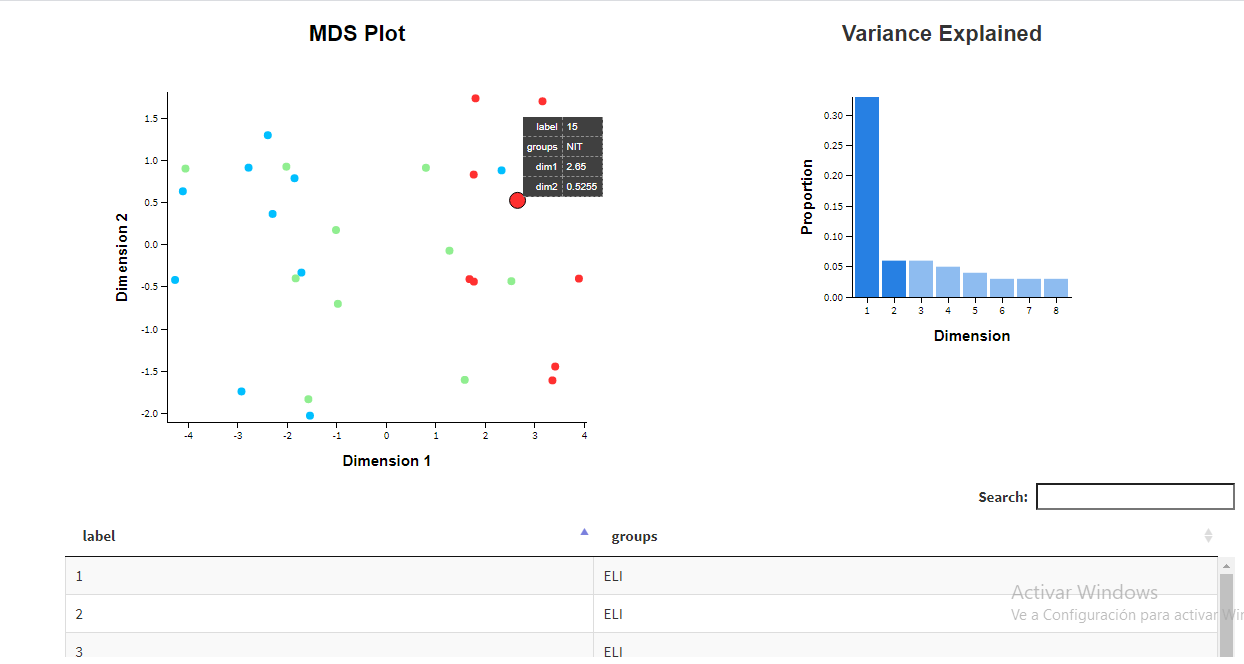
\includegraphics[width=1\linewidth]{C:/Pec2DatosOmicos/results/Glima1} \caption{Diagrama MDS interactivo}\label{fig:unnamed-chunk-12}
\end{figure}

La salida de glMDSPlot es una página html que muestra el diagrama MDS a
la izquierda y la cantidad de variación explicada por cada dimensión en
un diagrama de barras a la derecha. Podemos desplazarnos sobre los
puntos para encontrar información de la muestra y cambiar entre
dimensiones sucesivas en el diagrama MDS haciendo clic en las barras del
diagrama de barras.

\begin{Shaded}
\begin{Highlighting}[]
\NormalTok{logcounts <-}\StringTok{ }\KeywordTok{cpm}\NormalTok{(dgList, }\DataTypeTok{log=}\OtherTok{TRUE}\NormalTok{)}
\end{Highlighting}
\end{Shaded}

\hypertarget{normalizaciuxf3n-de-los-datos}{%
\subsubsection{Normalización de los
datos}\label{normalizaciuxf3n-de-los-datos}}

La función calcNormFactors de edgeR calcula los factores de
normalización entre bibliotecas.

\begin{Shaded}
\begin{Highlighting}[]
\NormalTok{dgList <-}\StringTok{ }\KeywordTok{calcNormFactors}\NormalTok{(dgList, }\DataTypeTok{method=}\StringTok{"TMM"}\NormalTok{)}
\end{Highlighting}
\end{Shaded}

Esto actualizará los factores de normalización del objeto dgList (sus
valores predeterminados son 1). veamos los factores de normalización
para las muestras.

Los factores de normalización multiplican a la unidad en todas las
bibliotecas. Un factor de normalización por debajo de uno indica que el
tamaño de la biblioteca se reducirá, ya que hay más supresión (es decir,
sesgo de composición) en esa biblioteca en relación con las otras
bibliotecas. Esto también es equivalente a escalar los recuentos hacia
arriba en esa muestra. Por el contrario, un factor superior a uno
aumenta el tamaño de la biblioteca y es equivalente a reducir los
recuentos.

La muestra GTEX.11DXX.0226.SM.5P9HL tiene el factor de normalización más
pequeño, y GTEX.13NZ9.1126.SM.5MR37 tiene el más grande. Si trazamos
gráficas de diferencia de medias usando la función plotMD para estas
muestras, deberíamos poder ver el problema de sesgo de composición.
Usaremos el logcounts, que se ha normalizado para el tamaño de la
biblioteca, pero no para el sesgo de composición.

\begin{Shaded}
\begin{Highlighting}[]
\NormalTok{logcounts <-}\StringTok{ }\KeywordTok{cpm}\NormalTok{(dgList,}\DataTypeTok{log=}\OtherTok{TRUE}\NormalTok{)}

\KeywordTok{par}\NormalTok{(}\DataTypeTok{mfrow=}\KeywordTok{c}\NormalTok{(}\DecValTok{1}\NormalTok{,}\DecValTok{2}\NormalTok{))}
\KeywordTok{plotMD}\NormalTok{(logcounts,}\DataTypeTok{column =} \DecValTok{5}\NormalTok{)}
\KeywordTok{abline}\NormalTok{(}\DataTypeTok{h=}\DecValTok{0}\NormalTok{,}\DataTypeTok{col=}\StringTok{"grey"}\NormalTok{)}
\KeywordTok{plotMD}\NormalTok{(logcounts,}\DataTypeTok{column =} \DecValTok{14}\NormalTok{)}
\KeywordTok{abline}\NormalTok{(}\DataTypeTok{h=}\DecValTok{0}\NormalTok{,}\DataTypeTok{col=}\StringTok{"grey"}\NormalTok{)}
\end{Highlighting}
\end{Shaded}

\includegraphics{RuizMacias_EvaM_PEC2_ADO_files/figure-latex/unnamed-chunk-15-1.pdf}

Los gráficos de diferencia de medias muestran la expresión promedio
(media: eje x) frente a log-fold-changes (diferencia: eje y). Veamos las
graficas con dgList:

\begin{Shaded}
\begin{Highlighting}[]
\KeywordTok{par}\NormalTok{(}\DataTypeTok{mfrow=}\KeywordTok{c}\NormalTok{(}\DecValTok{1}\NormalTok{,}\DecValTok{2}\NormalTok{))}
\KeywordTok{plotMD}\NormalTok{(dgList,}\DataTypeTok{column =} \DecValTok{5}\NormalTok{)}
\KeywordTok{abline}\NormalTok{(}\DataTypeTok{h=}\DecValTok{0}\NormalTok{,}\DataTypeTok{col=}\StringTok{"grey"}\NormalTok{)}
\KeywordTok{plotMD}\NormalTok{(dgList,}\DataTypeTok{column =} \DecValTok{14}\NormalTok{)}
\KeywordTok{abline}\NormalTok{(}\DataTypeTok{h=}\DecValTok{0}\NormalTok{,}\DataTypeTok{col=}\StringTok{"grey"}\NormalTok{)}
\end{Highlighting}
\end{Shaded}

\includegraphics{RuizMacias_EvaM_PEC2_ADO_files/figure-latex/unnamed-chunk-16-1.pdf}

\begin{Shaded}
\begin{Highlighting}[]
\KeywordTok{save}\NormalTok{(grupos,dgList,}\DataTypeTok{file=}\StringTok{"C:/Pec2DatosOmicos/results/preprocessing.Rdata"}\NormalTok{)}
\end{Highlighting}
\end{Shaded}

\hypertarget{expresiuxf3n-diferencial}{%
\subsubsection{Expresión diferencial}\label{expresiuxf3n-diferencial}}

\hypertarget{estimaciuxf3n-de-la-dispersiuxf3n}{%
\paragraph{Estimación de la
dispersión}\label{estimaciuxf3n-de-la-dispersiuxf3n}}

Un paso importante en el análisis de los datos DGE utilizando el modelo
NB es estimar el parámetro de dispersión para cada etiqueta, una medida
del grado de variación entre bibliotecas. La estimación de la dispersión
común da una idea de la variabilidad general a través del genoma para el
conjunto de datos.

Aquí vamos a hacer la estimación suponiendo que todo tiene la misma
dispersión común:

\begin{Shaded}
\begin{Highlighting}[]
\NormalTok{d1 <-}\StringTok{ }\KeywordTok{estimateCommonDisp}\NormalTok{(dgList, }\DataTypeTok{verbose=}\NormalTok{T)}
\end{Highlighting}
\end{Shaded}

\begin{verbatim}
## Disp = 0.2448 , BCV = 0.4948
\end{verbatim}

\begin{Shaded}
\begin{Highlighting}[]
\KeywordTok{names}\NormalTok{(d1)}
\end{Highlighting}
\end{Shaded}

\begin{verbatim}
## [1] "counts"            "samples"           "common.dispersion"
## [4] "pseudo.counts"     "pseudo.lib.size"   "AveLogCPM"
\end{verbatim}

Para el análisis de expresión diferencial, vamos a utilizar dispersiones
empíricas de Bayes. Hay que tener en cuenta que es necesario estimar la
dispersión común antes de estimar las dispersiones por etiquetas.

\begin{Shaded}
\begin{Highlighting}[]
\NormalTok{d1 <-}\StringTok{ }\KeywordTok{estimateTagwiseDisp}\NormalTok{(d1)}
\KeywordTok{names}\NormalTok{(d1)}
\end{Highlighting}
\end{Shaded}

\begin{verbatim}
##  [1] "counts"             "samples"            "common.dispersion" 
##  [4] "pseudo.counts"      "pseudo.lib.size"    "AveLogCPM"         
##  [7] "prior.df"           "prior.n"            "tagwise.dispersion"
## [10] "span"
\end{verbatim}

La función plotBCV() traza el coeficiente de variación biológica a nivel
de etiqueta (raíz cuadrada de dispersiones) frente a log2-CPM.

\begin{Shaded}
\begin{Highlighting}[]
\KeywordTok{plotBCV}\NormalTok{(d1)}
\end{Highlighting}
\end{Shaded}

\includegraphics{RuizMacias_EvaM_PEC2_ADO_files/figure-latex/unnamed-chunk-20-1.pdf}

Podemos ver que una sola estimación del coeficiente de variación no es
un buen modelo, ya que la dispersión aumenta a medida que aumenta el
recuento por millón (CPM).

Ahora calcularemos las estimaciones de dispersión con GLM:

Primero calcularemos la matriz de diseño:

\begin{Shaded}
\begin{Highlighting}[]
\NormalTok{designmat <-}\StringTok{ }\KeywordTok{model.matrix}\NormalTok{(}\OperatorTok{~}\StringTok{ }\DecValTok{0} \OperatorTok{+}\StringTok{ }\NormalTok{dgList}\OperatorTok{$}\NormalTok{samples}\OperatorTok{$}\NormalTok{group)}
\NormalTok{designmat}
\end{Highlighting}
\end{Shaded}

\begin{verbatim}
##    dgList$samples$groupELI dgList$samples$groupNIT dgList$samples$groupSFI
## 1                        1                       0                       0
## 2                        1                       0                       0
## 3                        1                       0                       0
## 4                        1                       0                       0
## 5                        1                       0                       0
## 6                        1                       0                       0
## 7                        1                       0                       0
## 8                        1                       0                       0
## 9                        1                       0                       0
## 10                       1                       0                       0
## 11                       0                       1                       0
## 12                       0                       1                       0
## 13                       0                       1                       0
## 14                       0                       1                       0
## 15                       0                       1                       0
## 16                       0                       1                       0
## 17                       0                       1                       0
## 18                       0                       1                       0
## 19                       0                       1                       0
## 20                       0                       1                       0
## 21                       0                       0                       1
## 22                       0                       0                       1
## 23                       0                       0                       1
## 24                       0                       0                       1
## 25                       0                       0                       1
## 26                       0                       0                       1
## 27                       0                       0                       1
## 28                       0                       0                       1
## 29                       0                       0                       1
## 30                       0                       0                       1
## attr(,"assign")
## [1] 1 1 1
## attr(,"contrasts")
## attr(,"contrasts")$`dgList$samples$group`
## [1] "contr.treatment"
\end{verbatim}

\begin{Shaded}
\begin{Highlighting}[]
\KeywordTok{colnames}\NormalTok{(designmat) <-}\StringTok{ }\KeywordTok{levels}\NormalTok{(dgList}\OperatorTok{$}\NormalTok{samples}\OperatorTok{$}\NormalTok{group)}
\end{Highlighting}
\end{Shaded}

La dispersión común estima el BCV general del conjunto de datos,
promediado sobre todos los genes.

\begin{Shaded}
\begin{Highlighting}[]
\NormalTok{d2 <-}\StringTok{ }\KeywordTok{estimateGLMCommonDisp}\NormalTok{(dgList,designmat)}
\end{Highlighting}
\end{Shaded}

Ahora haremos las estimaciones de dispersión delos genes:

\begin{Shaded}
\begin{Highlighting}[]
\NormalTok{d2 <-}\StringTok{ }\KeywordTok{estimateGLMCommonDisp}\NormalTok{(dgList,designmat)}
\NormalTok{d2 <-}\StringTok{ }\KeywordTok{estimateGLMTrendedDisp}\NormalTok{(d2,designmat)}
\CommentTok{# podemos usar el metodo "auto", "bin.spline", "power", "spline", "bin.loess"}

\NormalTok{d2 <-}\StringTok{ }\KeywordTok{estimateGLMTagwiseDisp}\NormalTok{(d2,designmat)}
\end{Highlighting}
\end{Shaded}

Hacemos una gráfica de las dispersiones estimadas:

\begin{Shaded}
\begin{Highlighting}[]
\KeywordTok{plotBCV}\NormalTok{(d2)}
\end{Highlighting}
\end{Shaded}

\includegraphics{RuizMacias_EvaM_PEC2_ADO_files/figure-latex/unnamed-chunk-24-1.pdf}

\hypertarget{comparacion-entre-los-modelos-deseq-y-edger}{%
\paragraph{Comparacion entre los modelos DESeq y
edgeR}\label{comparacion-entre-los-modelos-deseq-y-edger}}

Veamos los resultados usando DESeq:

\begin{Shaded}
\begin{Highlighting}[]
\NormalTok{cds <-}\StringTok{ }\KeywordTok{newCountDataSet}\NormalTok{(}\KeywordTok{data.frame}\NormalTok{(dgList}\OperatorTok{$}\NormalTok{counts), dgList}\OperatorTok{$}\NormalTok{samples}\OperatorTok{$}\NormalTok{group)}
\NormalTok{cds <-}\StringTok{ }\KeywordTok{estimateSizeFactors}\NormalTok{(cds)}
\KeywordTok{sizeFactors}\NormalTok{(cds)}
\end{Highlighting}
\end{Shaded}

\begin{verbatim}
##  GTEX.ZYY3.1926.SM.5GZXS  GTEX.YJ89.0726.SM.5P9F7 GTEX.11XUK.0226.SM.5EQLW 
##                0.9127543                1.5656968                0.9414113 
##  GTEX.YFC4.2626.SM.5P9FQ GTEX.13NZ9.1126.SM.5MR37  GTEX.R55G.0726.SM.2TC6J 
##                1.7190780                1.3531099                0.3086861 
##  GTEX.PLZ4.1226.SM.2I5FE  GTEX.TMMY.0826.SM.33HB9 GTEX.14AS3.0226.SM.5Q5B6 
##                1.2616073                1.4984118                0.8923937 
## GTEX.13QJC.0826.SM.5RQKC  GTEX.QV31.0726.SM.3GAEG GTEX.13OW7.0826.SM.5L3EL 
##                0.9414876                0.9125279                0.8237525 
##  GTEX.X8HC.0726.SM.46MWG GTEX.11DXX.0226.SM.5P9HL  GTEX.Q734.0526.SM.2I3EH 
##                0.9628535                1.4468140                1.0157057 
## GTEX.13113.0126.SM.5LZVX  GTEX.R3RS.0726.SM.3GIJR GTEX.13S86.1126.SM.5RQJX 
##                0.8509219                0.2428189                0.7229740 
## GTEX.13FTY.0726.SM.5J2OH  GTEX.ZYFC.0926.SM.5GZWW  GTEX.QLQ7.0726.SM.2I5G2 
##                1.1876266                0.9899802                1.4854682 
##  GTEX.ZLV1.0126.SM.4WWBZ  GTEX.Y5V6.0526.SM.4VBRV GTEX.13FH7.0126.SM.5KLZ1 
##                1.0337837                1.2211305                1.2135299 
## GTEX.13NZ8.0226.SM.5J2OK  GTEX.R55C.0626.SM.2TF4Q  GTEX.WYVS.0326.SM.3NM9V 
##                1.1958195                0.7654034                1.5291694 
## GTEX.131YS.0726.SM.5P9G9 GTEX.11GS4.0826.SM.5986J GTEX.13FXS.0726.SM.5LZXJ 
##                1.3806445                0.9543062                0.9532746
\end{verbatim}

\begin{Shaded}
\begin{Highlighting}[]
\NormalTok{cds <-}\StringTok{ }\KeywordTok{estimateDispersions}\NormalTok{( cds , }\DataTypeTok{method=}\StringTok{"blind"}\NormalTok{)}
\KeywordTok{plotDispEsts}\NormalTok{(cds)}
\end{Highlighting}
\end{Shaded}

\includegraphics{RuizMacias_EvaM_PEC2_ADO_files/figure-latex/unnamed-chunk-25-1.pdf}

En este gráfico se traza la dispersión en el eje vertical en lugar del
coeficiente de variación biológica.

\hypertarget{expresiuxf3n-diferencial-1}{%
\paragraph{Expresión diferencial}\label{expresiuxf3n-diferencial-1}}

Una vez que se estiman las dispersiones, podemos proceder con los
procedimientos de prueba para determinar la expresión diferencial. La
función exactTest()lleva a cabo pruebas con etiquetas usando la prueba
binomial negativa exacta. La topTags()función muestra los resultados de
las pruebas para las n etiquetas más significativas . Por defecto, el
algoritmo de Benjamini y Hochberg se usa para controlar los FDR.

Primero lo haremos para d1 en el que solo habia una dispersión comun:

\begin{Shaded}
\begin{Highlighting}[]
\NormalTok{et12 <-}\StringTok{ }\KeywordTok{exactTest}\NormalTok{(d1, }\DataTypeTok{pair=}\KeywordTok{c}\NormalTok{(}\DecValTok{1}\NormalTok{,}\DecValTok{2}\NormalTok{)) }\CommentTok{# compara grupos 1 y 2}
\NormalTok{et13 <-}\StringTok{ }\KeywordTok{exactTest}\NormalTok{(d1, }\DataTypeTok{pair=}\KeywordTok{c}\NormalTok{(}\DecValTok{1}\NormalTok{,}\DecValTok{3}\NormalTok{)) }\CommentTok{# compara grupos 1 y 3}
\NormalTok{et23 <-}\StringTok{ }\KeywordTok{exactTest}\NormalTok{(d1, }\DataTypeTok{pair=}\KeywordTok{c}\NormalTok{(}\DecValTok{2}\NormalTok{,}\DecValTok{3}\NormalTok{)) }\CommentTok{# compara grupos 2 y 3}

\KeywordTok{topTags}\NormalTok{(et12)}
\end{Highlighting}
\end{Shaded}

\begin{verbatim}
## Comparison of groups:  NIT-ELI 
##                     logFC   logCPM       PValue          FDR
## ENSG00000105369 -7.959291 5.370352 1.503462e-18 1.656635e-14
## ENSG00000083454 -6.724115 4.610802 1.586068e-18 1.656635e-14
## ENSG00000143297 -7.039446 5.235187 2.258843e-18 1.656635e-14
## ENSG00000136573 -7.100350 4.633171 7.348041e-18 4.041790e-14
## ENSG00000035720 -6.931713 1.704583 2.991016e-17 1.316167e-13
## ENSG00000132704 -8.095621 3.776334 6.126310e-17 2.246518e-13
## ENSG00000211893 -7.432055 8.143807 8.949981e-17 2.813107e-13
## ENSG00000132465 -6.159953 7.569634 2.258388e-16 6.211131e-13
## ENSG00000110777 -6.075717 5.478448 3.502111e-16 7.728291e-13
## ENSG00000174123 -6.452497 3.312477 3.578128e-16 7.728291e-13
\end{verbatim}

\begin{Shaded}
\begin{Highlighting}[]
\KeywordTok{topTags}\NormalTok{(et13)}
\end{Highlighting}
\end{Shaded}

\begin{verbatim}
## Comparison of groups:  SFI-ELI 
##                      logFC     logCPM       PValue          FDR
## ENSG00000152952  1.1579954  6.5928899 5.499935e-09 0.0001210096
## ENSG00000114270 -2.1261371  4.0917445 3.601060e-08 0.0003961526
## ENSG00000164638  1.8385594  4.4874509 9.217038e-08 0.0006139220
## ENSG00000246575 -1.5595843  0.8116396 1.116120e-07 0.0006139220
## ENSG00000230937 -3.3454314  0.1182087 1.864241e-07 0.0007186033
## ENSG00000235111 -1.9815532  0.6971040 1.959649e-07 0.0007186033
## ENSG00000117450  1.0882947  8.6060029 3.322718e-07 0.0010443776
## ENSG00000254029 -6.2054585 -1.7146513 4.153228e-07 0.0011422416
## ENSG00000164023  1.1871192  5.0832377 5.131068e-07 0.0011528167
## ENSG00000091164  0.8840216  7.0897588 5.239600e-07 0.0011528167
\end{verbatim}

\begin{Shaded}
\begin{Highlighting}[]
\KeywordTok{topTags}\NormalTok{(et23)}
\end{Highlighting}
\end{Shaded}

\begin{verbatim}
## Comparison of groups:  SFI-NIT 
##                    logFC   logCPM       PValue          FDR
## ENSG00000132465 5.790584 7.569634 4.212307e-15 9.267917e-11
## ENSG00000211900 6.861673 3.418219 2.019553e-14 1.929256e-10
## ENSG00000105369 6.422645 5.370352 3.410472e-14 1.929256e-10
## ENSG00000211966 7.148734 4.607411 3.507420e-14 1.929256e-10
## ENSG00000211598 6.961605 6.072348 5.262867e-14 2.315872e-10
## ENSG00000211947 6.780802 4.162516 8.061528e-14 2.956162e-10
## ENSG00000240041 6.436346 3.953837 1.097040e-13 3.190175e-10
## ENSG00000211935 7.793636 3.096525 1.180827e-13 3.190175e-10
## ENSG00000242887 6.820799 2.397691 1.306763e-13 3.190175e-10
## ENSG00000241351 6.807645 5.966672 1.449948e-13 3.190175e-10
\end{verbatim}

El número total de genes expresados diferencialmente en FDR
\textless0.05 es:

\begin{Shaded}
\begin{Highlighting}[]
\NormalTok{de12 <-}\StringTok{ }\KeywordTok{decideTestsDGE}\NormalTok{(et12, }\DataTypeTok{adjust.method=}\StringTok{"BH"}\NormalTok{, }\DataTypeTok{p.value=}\FloatTok{0.05}\NormalTok{)}
\NormalTok{de13 <-}\StringTok{ }\KeywordTok{decideTestsDGE}\NormalTok{(et13, }\DataTypeTok{adjust.method=}\StringTok{"BH"}\NormalTok{, }\DataTypeTok{p.value=}\FloatTok{0.05}\NormalTok{)}
\NormalTok{de23 <-}\StringTok{ }\KeywordTok{decideTestsDGE}\NormalTok{(et23, }\DataTypeTok{adjust.method=}\StringTok{"BH"}\NormalTok{, }\DataTypeTok{p.value=}\FloatTok{0.05}\NormalTok{)}
\KeywordTok{summary}\NormalTok{(de12)}
\end{Highlighting}
\end{Shaded}

\begin{verbatim}
##        NIT-ELI
## Down      2109
## NotSig   19051
## Up         842
\end{verbatim}

\begin{Shaded}
\begin{Highlighting}[]
\KeywordTok{summary}\NormalTok{(de13)}
\end{Highlighting}
\end{Shaded}

\begin{verbatim}
##        SFI-ELI
## Down       775
## NotSig   20580
## Up         647
\end{verbatim}

\begin{Shaded}
\begin{Highlighting}[]
\KeywordTok{summary}\NormalTok{(de23)}
\end{Highlighting}
\end{Shaded}

\begin{verbatim}
##        SFI-NIT
## Down        30
## NotSig   21411
## Up         561
\end{verbatim}

Se nos muestran las etiquetas infraexpresadas, no expresadas
diferencialmente y sobreexpresadas, respectivamente.

\begin{Shaded}
\begin{Highlighting}[]
\NormalTok{de12tags12 <-}\StringTok{ }\KeywordTok{rownames}\NormalTok{(d1)[}\KeywordTok{as.logical}\NormalTok{(de12)]}
\NormalTok{de13tags13 <-}\StringTok{ }\KeywordTok{rownames}\NormalTok{(d1)[}\KeywordTok{as.logical}\NormalTok{(de13)]}
\NormalTok{de23tags23 <-}\StringTok{ }\KeywordTok{rownames}\NormalTok{(d1)[}\KeywordTok{as.logical}\NormalTok{(de23)]}
\KeywordTok{plotSmear}\NormalTok{(et12, }\DataTypeTok{de.tags=}\NormalTok{de12tags12)}
\KeywordTok{abline}\NormalTok{(}\DataTypeTok{h =} \KeywordTok{c}\NormalTok{(}\OperatorTok{-}\DecValTok{2}\NormalTok{, }\DecValTok{2}\NormalTok{), }\DataTypeTok{col =} \StringTok{"blue"}\NormalTok{)}
\end{Highlighting}
\end{Shaded}

\includegraphics{RuizMacias_EvaM_PEC2_ADO_files/figure-latex/unnamed-chunk-28-1.pdf}

\begin{Shaded}
\begin{Highlighting}[]
\KeywordTok{plotSmear}\NormalTok{(et13, }\DataTypeTok{de.tags=}\NormalTok{de13tags13)}
\KeywordTok{abline}\NormalTok{(}\DataTypeTok{h =} \KeywordTok{c}\NormalTok{(}\OperatorTok{-}\DecValTok{2}\NormalTok{, }\DecValTok{2}\NormalTok{), }\DataTypeTok{col =} \StringTok{"blue"}\NormalTok{)}
\end{Highlighting}
\end{Shaded}

\includegraphics{RuizMacias_EvaM_PEC2_ADO_files/figure-latex/unnamed-chunk-28-2.pdf}

\begin{Shaded}
\begin{Highlighting}[]
\KeywordTok{plotSmear}\NormalTok{(et23, }\DataTypeTok{de.tags=}\NormalTok{de23tags23)}
\KeywordTok{abline}\NormalTok{(}\DataTypeTok{h =} \KeywordTok{c}\NormalTok{(}\OperatorTok{-}\DecValTok{2}\NormalTok{, }\DecValTok{2}\NormalTok{), }\DataTypeTok{col =} \StringTok{"blue"}\NormalTok{)}
\end{Highlighting}
\end{Shaded}

\includegraphics{RuizMacias_EvaM_PEC2_ADO_files/figure-latex/unnamed-chunk-28-3.pdf}

Ahora haremos la expresion diferencial con GLM (d2).

Ajustamos el modelo lineal

\begin{Shaded}
\begin{Highlighting}[]
\NormalTok{fit <-}\StringTok{ }\KeywordTok{glmFit}\NormalTok{(d2, designmat)}
\KeywordTok{names}\NormalTok{(fit)}
\end{Highlighting}
\end{Shaded}

\begin{verbatim}
##  [1] "coefficients"          "fitted.values"         "deviance"             
##  [4] "method"                "counts"                "unshrunk.coefficients"
##  [7] "df.residual"           "design"                "offset"               
## [10] "dispersion"            "prior.count"           "samples"              
## [13] "prior.df"              "AveLogCPM"
\end{verbatim}

\begin{Shaded}
\begin{Highlighting}[]
\KeywordTok{head}\NormalTok{(}\KeywordTok{coef}\NormalTok{(fit))}
\end{Highlighting}
\end{Shaded}

\begin{verbatim}
##                       ELI       NIT       SFI
## ENSG00000227232 -11.17795 -11.10555 -11.18483
## ENSG00000233750 -13.54019 -14.29986 -14.58753
## ENSG00000237683 -11.13330 -10.82992 -11.36526
## ENSG00000239906 -15.40420 -14.93073 -15.53459
## ENSG00000241860 -13.17183 -13.16994 -13.56915
## ENSG00000228463 -14.04140 -14.01043 -13.81948
\end{verbatim}

Realizamos las pruebas y le decimos que muestre los genes principales:

\begin{Shaded}
\begin{Highlighting}[]
\NormalTok{lrt12 <-}\StringTok{ }\KeywordTok{glmLRT}\NormalTok{(fit, }\DataTypeTok{contrast=}\KeywordTok{c}\NormalTok{(}\DecValTok{1}\NormalTok{,}\OperatorTok{-}\DecValTok{1}\NormalTok{,}\DecValTok{0}\NormalTok{))}
\NormalTok{lrt13 <-}\StringTok{ }\KeywordTok{glmLRT}\NormalTok{(fit, }\DataTypeTok{contrast=}\KeywordTok{c}\NormalTok{(}\DecValTok{1}\NormalTok{,}\DecValTok{0}\NormalTok{,}\OperatorTok{-}\DecValTok{1}\NormalTok{))}
\NormalTok{lrt23 <-}\StringTok{ }\KeywordTok{glmLRT}\NormalTok{(fit, }\DataTypeTok{contrast=}\KeywordTok{c}\NormalTok{(}\DecValTok{0}\NormalTok{,}\DecValTok{1}\NormalTok{,}\OperatorTok{-}\DecValTok{1}\NormalTok{))}
\KeywordTok{topTags}\NormalTok{(lrt12)}
\end{Highlighting}
\end{Shaded}

\begin{verbatim}
## Coefficient:  1*ELI -1*NIT 
##                    logFC   logCPM       LR       PValue          FDR
## ENSG00000083454 6.724404 4.610790 78.06307 9.980274e-19 8.075012e-15
## ENSG00000105369 7.959764 5.370352 78.01250 1.023908e-18 8.075012e-15
## ENSG00000143297 7.039684 5.235190 77.86904 1.101038e-18 8.075012e-15
## ENSG00000136573 7.100830 4.633165 74.48283 6.116809e-18 3.364551e-14
## ENSG00000035720 6.934206 1.704591 71.63180 2.593436e-17 1.141215e-13
## ENSG00000132704 8.096907 3.776319 70.91064 3.737766e-17 1.370639e-13
## ENSG00000211893 7.432092 8.143808 69.91506 6.191385e-17 1.946041e-13
## ENSG00000132465 6.159986 7.569635 68.39030 1.341358e-16 3.689069e-13
## ENSG00000110777 6.075844 5.478449 67.92249 1.700505e-16 4.157169e-13
## ENSG00000174123 6.453040 3.312501 67.50060 2.106227e-16 4.634120e-13
\end{verbatim}

\begin{Shaded}
\begin{Highlighting}[]
\KeywordTok{topTags}\NormalTok{(lrt13)}
\end{Highlighting}
\end{Shaded}

\begin{verbatim}
## Coefficient:  1*ELI -1*SFI 
##                      logFC    logCPM       LR       PValue          FDR
## ENSG00000152952 -1.1579906 6.5928896 34.53262 4.191668e-09 9.222508e-05
## ENSG00000114270  2.1261204 4.0917531 31.39518 2.105025e-08 2.315738e-04
## ENSG00000164638 -1.8385325 4.4874560 29.09864 6.878522e-08 5.044708e-04
## ENSG00000246575  1.5594593 0.8116321 28.03271 1.192823e-07 5.559205e-04
## ENSG00000230937  3.3445600 0.1184788 27.92156 1.263341e-07 5.559205e-04
## ENSG00000235111  1.9813407 0.6971852 27.30972 1.733381e-07 6.356308e-04
## ENSG00000164023 -1.1871107 5.0832415 25.63372 4.127637e-07 1.084353e-03
## ENSG00000091164 -0.8840174 7.0897583 25.50468 4.413103e-07 1.084353e-03
## ENSG00000065833 -1.6544754 4.0982129 25.38601 4.693100e-07 1.084353e-03
## ENSG00000011201 -0.9262465 4.3598616 25.28759 4.938759e-07 1.084353e-03
\end{verbatim}

\begin{Shaded}
\begin{Highlighting}[]
\KeywordTok{topTags}\NormalTok{(lrt23)}
\end{Highlighting}
\end{Shaded}

\begin{verbatim}
## Coefficient:  1*NIT -1*SFI 
##                     logFC   logCPM       LR       PValue          FDR
## ENSG00000132465 -5.790607 7.569635 62.55978 2.584785e-15 5.687044e-11
## ENSG00000211900 -6.862566 3.418238 59.51218 1.215397e-14 1.337058e-10
## ENSG00000105369 -6.422998 5.370352 58.12292 2.462403e-14 1.728339e-10
## ENSG00000211966 -7.149144 4.607428 57.41076 3.536664e-14 1.728339e-10
## ENSG00000254395 -8.444301 1.032817 57.20451 3.927686e-14 1.728339e-10
## ENSG00000211598 -6.961892 6.072352 56.70652 5.059563e-14 1.786294e-10
## ENSG00000211947 -6.780567 4.162529 56.21467 6.497487e-14 1.786294e-10
## ENSG00000240041 -6.436744 3.953852 56.14523 6.731065e-14 1.786294e-10
## ENSG00000211935 -7.795932 3.096583 55.98384 7.306903e-14 1.786294e-10
## ENSG00000241351 -6.807787 5.966674 55.60578 8.856266e-14 1.948556e-10
\end{verbatim}

El número total de genes expresados diferencialmente en FDR
\textless0.05 es:

\begin{Shaded}
\begin{Highlighting}[]
\NormalTok{de2en <-}\StringTok{ }\KeywordTok{decideTestsDGE}\NormalTok{(lrt12, }\DataTypeTok{adjust.method=}\StringTok{"BH"}\NormalTok{, }\DataTypeTok{p.value =} \FloatTok{0.05}\NormalTok{)}
\NormalTok{de2es <-}\StringTok{ }\KeywordTok{decideTestsDGE}\NormalTok{(lrt13, }\DataTypeTok{adjust.method=}\StringTok{"BH"}\NormalTok{, }\DataTypeTok{p.value =} \FloatTok{0.05}\NormalTok{)}
\NormalTok{de2ns <-}\StringTok{ }\KeywordTok{decideTestsDGE}\NormalTok{(lrt23, }\DataTypeTok{adjust.method=}\StringTok{"BH"}\NormalTok{, }\DataTypeTok{p.value =} \FloatTok{0.05}\NormalTok{)}
\NormalTok{de2tagsen <-}\StringTok{ }\KeywordTok{rownames}\NormalTok{(d2)[}\KeywordTok{as.logical}\NormalTok{(de2en)]}
\NormalTok{de2tagses <-}\StringTok{ }\KeywordTok{rownames}\NormalTok{(d2)[}\KeywordTok{as.logical}\NormalTok{(de2es)]}
\NormalTok{de2tagsns <-}\StringTok{ }\KeywordTok{rownames}\NormalTok{(d2)[}\KeywordTok{as.logical}\NormalTok{(de2ns)]}
\KeywordTok{summary}\NormalTok{(de2en)}
\end{Highlighting}
\end{Shaded}

\begin{verbatim}
##        1*ELI -1*NIT
## Down            876
## NotSig        18999
## Up             2127
\end{verbatim}

\begin{Shaded}
\begin{Highlighting}[]
\KeywordTok{summary}\NormalTok{(de2es)}
\end{Highlighting}
\end{Shaded}

\begin{verbatim}
##        1*ELI -1*SFI
## Down            674
## NotSig        20521
## Up              807
\end{verbatim}

\begin{Shaded}
\begin{Highlighting}[]
\KeywordTok{summary}\NormalTok{(de2ns)}
\end{Highlighting}
\end{Shaded}

\begin{verbatim}
##        1*NIT -1*SFI
## Down            561
## NotSig        21410
## Up               31
\end{verbatim}

Veamos ahora los graficos para cada contraste:

\begin{Shaded}
\begin{Highlighting}[]
\KeywordTok{plotSmear}\NormalTok{(lrt12, }\DataTypeTok{de.tags=}\NormalTok{de2tagsen)}
\KeywordTok{abline}\NormalTok{(}\DataTypeTok{h =} \KeywordTok{c}\NormalTok{(}\OperatorTok{-}\DecValTok{2}\NormalTok{, }\DecValTok{2}\NormalTok{), }\DataTypeTok{col =} \StringTok{"blue"}\NormalTok{)}
\end{Highlighting}
\end{Shaded}

\includegraphics{RuizMacias_EvaM_PEC2_ADO_files/figure-latex/unnamed-chunk-32-1.pdf}

\begin{Shaded}
\begin{Highlighting}[]
\KeywordTok{plotSmear}\NormalTok{(lrt13, }\DataTypeTok{de.tags=}\NormalTok{de2tagses)}
\KeywordTok{abline}\NormalTok{(}\DataTypeTok{h =} \KeywordTok{c}\NormalTok{(}\OperatorTok{-}\DecValTok{2}\NormalTok{, }\DecValTok{2}\NormalTok{), }\DataTypeTok{col =} \StringTok{"blue"}\NormalTok{)}
\end{Highlighting}
\end{Shaded}

\includegraphics{RuizMacias_EvaM_PEC2_ADO_files/figure-latex/unnamed-chunk-32-2.pdf}

\begin{Shaded}
\begin{Highlighting}[]
\KeywordTok{plotSmear}\NormalTok{(lrt23, }\DataTypeTok{de.tags=}\NormalTok{de2tagsns)}
\KeywordTok{abline}\NormalTok{(}\DataTypeTok{h =} \KeywordTok{c}\NormalTok{(}\OperatorTok{-}\DecValTok{2}\NormalTok{, }\DecValTok{2}\NormalTok{), }\DataTypeTok{col =} \StringTok{"blue"}\NormalTok{)}
\end{Highlighting}
\end{Shaded}

\includegraphics{RuizMacias_EvaM_PEC2_ADO_files/figure-latex/unnamed-chunk-32-3.pdf}

\begin{Shaded}
\begin{Highlighting}[]
\NormalTok{results <-}\StringTok{ }\KeywordTok{as.data.frame}\NormalTok{(}\KeywordTok{topTags}\NormalTok{(lrt12,}\DataTypeTok{n =} \OtherTok{Inf}\NormalTok{))}
\KeywordTok{head}\NormalTok{(results)}
\end{Highlighting}
\end{Shaded}

\begin{verbatim}
##                    logFC   logCPM       LR       PValue          FDR
## ENSG00000083454 6.724404 4.610790 78.06307 9.980274e-19 8.075012e-15
## ENSG00000105369 7.959764 5.370352 78.01250 1.023908e-18 8.075012e-15
## ENSG00000143297 7.039684 5.235190 77.86904 1.101038e-18 8.075012e-15
## ENSG00000136573 7.100830 4.633165 74.48283 6.116809e-18 3.364551e-14
## ENSG00000035720 6.934206 1.704591 71.63180 2.593436e-17 1.141215e-13
## ENSG00000132704 8.096907 3.776319 70.91064 3.737766e-17 1.370639e-13
\end{verbatim}

\begin{Shaded}
\begin{Highlighting}[]
\KeywordTok{dim}\NormalTok{(results)}
\end{Highlighting}
\end{Shaded}

\begin{verbatim}
## [1] 22002     5
\end{verbatim}

\begin{Shaded}
\begin{Highlighting}[]
\NormalTok{results2 <-}\StringTok{ }\KeywordTok{as.data.frame}\NormalTok{(}\KeywordTok{topTags}\NormalTok{(lrt13,}\DataTypeTok{n =} \OtherTok{Inf}\NormalTok{))}
\KeywordTok{head}\NormalTok{(results2)}
\end{Highlighting}
\end{Shaded}

\begin{verbatim}
##                     logFC    logCPM       LR       PValue          FDR
## ENSG00000152952 -1.157991 6.5928896 34.53262 4.191668e-09 9.222508e-05
## ENSG00000114270  2.126120 4.0917531 31.39518 2.105025e-08 2.315738e-04
## ENSG00000164638 -1.838532 4.4874560 29.09864 6.878522e-08 5.044708e-04
## ENSG00000246575  1.559459 0.8116321 28.03271 1.192823e-07 5.559205e-04
## ENSG00000230937  3.344560 0.1184788 27.92156 1.263341e-07 5.559205e-04
## ENSG00000235111  1.981341 0.6971852 27.30972 1.733381e-07 6.356308e-04
\end{verbatim}

\begin{Shaded}
\begin{Highlighting}[]
\KeywordTok{dim}\NormalTok{(results2)}
\end{Highlighting}
\end{Shaded}

\begin{verbatim}
## [1] 22002     5
\end{verbatim}

\begin{Shaded}
\begin{Highlighting}[]
\NormalTok{results3 <-}\StringTok{ }\KeywordTok{as.data.frame}\NormalTok{(}\KeywordTok{topTags}\NormalTok{(lrt23,}\DataTypeTok{n =} \OtherTok{Inf}\NormalTok{))}
\KeywordTok{head}\NormalTok{(results3)}
\end{Highlighting}
\end{Shaded}

\begin{verbatim}
##                     logFC   logCPM       LR       PValue          FDR
## ENSG00000132465 -5.790607 7.569635 62.55978 2.584785e-15 5.687044e-11
## ENSG00000211900 -6.862566 3.418238 59.51218 1.215397e-14 1.337058e-10
## ENSG00000105369 -6.422998 5.370352 58.12292 2.462403e-14 1.728339e-10
## ENSG00000211966 -7.149144 4.607428 57.41076 3.536664e-14 1.728339e-10
## ENSG00000254395 -8.444301 1.032817 57.20451 3.927686e-14 1.728339e-10
## ENSG00000211598 -6.961892 6.072352 56.70652 5.059563e-14 1.786294e-10
\end{verbatim}

\begin{Shaded}
\begin{Highlighting}[]
\KeywordTok{dim}\NormalTok{(results3)}
\end{Highlighting}
\end{Shaded}

\begin{verbatim}
## [1] 22002     5
\end{verbatim}

\begin{Shaded}
\begin{Highlighting}[]
\KeywordTok{summary}\NormalTok{(de <-}\StringTok{ }\KeywordTok{decideTestsDGE}\NormalTok{(lrt12,}
                             \DataTypeTok{adjust.method=}\StringTok{"BH"}\NormalTok{, }\DataTypeTok{p.value =} \FloatTok{0.05}\NormalTok{))}
\end{Highlighting}
\end{Shaded}

\begin{verbatim}
##        1*ELI -1*NIT
## Down            876
## NotSig        18999
## Up             2127
\end{verbatim}

\begin{Shaded}
\begin{Highlighting}[]
\KeywordTok{save}\NormalTok{(lrt12,}
\NormalTok{     lrt13,}
\NormalTok{     lrt23,}
\NormalTok{     dgList,grupos,}\DataTypeTok{file=}\StringTok{"C:/Pec2DatosOmicos/results/DE.Rdata"}\NormalTok{)}
\end{Highlighting}
\end{Shaded}

\hypertarget{anotaciuxf3n-y-visualizaciuxf3n-de-resultados}{%
\paragraph{Anotación y visualización de
resultados}\label{anotaciuxf3n-y-visualizaciuxf3n-de-resultados}}

Para anotar nuestros resultados, vamos a quedarnos con los símbolos
genéticos y el nombre completo del gen. Separaremos la información de
anotación en un marco de datos usando la funcion select.

Ajunto el codigo de results2 y results3 en el apendice.

\begin{Shaded}
\begin{Highlighting}[]
\NormalTok{ann <-}\StringTok{ }\KeywordTok{select}\NormalTok{(org.Hs.eg.db,}\DataTypeTok{keys=}\KeywordTok{rownames}\NormalTok{(results), }\DataTypeTok{keytype =} \StringTok{"ENSEMBL"}\NormalTok{,}
              \DataTypeTok{columns=}\KeywordTok{c}\NormalTok{(}\StringTok{"SYMBOL"}\NormalTok{,}\StringTok{"GENENAME"}\NormalTok{))}
\end{Highlighting}
\end{Shaded}

\begin{verbatim}
## 'select()' returned 1:many mapping between keys and columns
\end{verbatim}

\begin{Shaded}
\begin{Highlighting}[]
\KeywordTok{head}\NormalTok{(ann)}
\end{Highlighting}
\end{Shaded}

\begin{verbatim}
##           ENSEMBL SYMBOL                                       GENENAME
## 1 ENSG00000083454  P2RX5                      purinergic receptor P2X 5
## 2 ENSG00000105369  CD79A                                 CD79a molecule
## 3 ENSG00000143297  FCRL5                             Fc receptor like 5
## 4 ENSG00000136573    BLK BLK proto-oncogene, Src family tyrosine kinase
## 5 ENSG00000035720  STAP1     signal transducing adaptor family member 1
## 6 ENSG00000132704  FCRL2                             Fc receptor like 2
\end{verbatim}

\begin{Shaded}
\begin{Highlighting}[]
\KeywordTok{dim}\NormalTok{(ann)}
\end{Highlighting}
\end{Shaded}

\begin{verbatim}
## [1] 22143     3
\end{verbatim}

\begin{verbatim}
## 'select()' returned 1:many mapping between keys and columns
## 'select()' returned 1:many mapping between keys and columns
\end{verbatim}

Verifiquemos nuevamente que la columna ENSEMBL coincida exactamente con
los nombres de las filas de results.

\begin{Shaded}
\begin{Highlighting}[]
\KeywordTok{table}\NormalTok{(}\KeywordTok{unique}\NormalTok{(ann}\OperatorTok{$}\NormalTok{ENSEMBL)}\OperatorTok{==}\KeywordTok{rownames}\NormalTok{(results))}
\end{Highlighting}
\end{Shaded}

\begin{verbatim}
## 
##  TRUE 
## 22002
\end{verbatim}

\begin{Shaded}
\begin{Highlighting}[]
\CommentTok{# Tengo que hacer esto debido a la salida 'select()' returned 1:many...}
\NormalTok{ann <-}\StringTok{ }\NormalTok{ann[}\OperatorTok{!}\KeywordTok{duplicated}\NormalTok{(ann}\OperatorTok{$}\NormalTok{ENSEMBL), ] }
\NormalTok{results.annotated <-}\StringTok{ }\KeywordTok{cbind}\NormalTok{(results, ann)}

\KeywordTok{head}\NormalTok{(results.annotated)}
\end{Highlighting}
\end{Shaded}

\begin{verbatim}
##                    logFC   logCPM       LR       PValue          FDR
## ENSG00000083454 6.724404 4.610790 78.06307 9.980274e-19 8.075012e-15
## ENSG00000105369 7.959764 5.370352 78.01250 1.023908e-18 8.075012e-15
## ENSG00000143297 7.039684 5.235190 77.86904 1.101038e-18 8.075012e-15
## ENSG00000136573 7.100830 4.633165 74.48283 6.116809e-18 3.364551e-14
## ENSG00000035720 6.934206 1.704591 71.63180 2.593436e-17 1.141215e-13
## ENSG00000132704 8.096907 3.776319 70.91064 3.737766e-17 1.370639e-13
##                         ENSEMBL SYMBOL
## ENSG00000083454 ENSG00000083454  P2RX5
## ENSG00000105369 ENSG00000105369  CD79A
## ENSG00000143297 ENSG00000143297  FCRL5
## ENSG00000136573 ENSG00000136573    BLK
## ENSG00000035720 ENSG00000035720  STAP1
## ENSG00000132704 ENSG00000132704  FCRL2
##                                                       GENENAME
## ENSG00000083454                      purinergic receptor P2X 5
## ENSG00000105369                                 CD79a molecule
## ENSG00000143297                             Fc receptor like 5
## ENSG00000136573 BLK proto-oncogene, Src family tyrosine kinase
## ENSG00000035720     signal transducing adaptor family member 1
## ENSG00000132704                             Fc receptor like 2
\end{verbatim}

\begin{Shaded}
\begin{Highlighting}[]
\KeywordTok{write.csv}\NormalTok{(results.annotated,}\DataTypeTok{file=}\StringTok{"C:/Pec2DatosOmicos/results/ELIVsNIT.csv"}\NormalTok{,}
          \DataTypeTok{row.names=}\OtherTok{FALSE}\NormalTok{)}
\end{Highlighting}
\end{Shaded}

Una alternativa es utilizar BioMart . BioMart es mucho más completo,
pero los ``organism packages'' se ajustan mejor al flujo de trabajo de
Bioconductor.

Veamos también como queda representado con un VolcanoPlot:

\begin{Shaded}
\begin{Highlighting}[]
\NormalTok{detags <-}\StringTok{ }\KeywordTok{rownames}\NormalTok{(dgList)[}\KeywordTok{as.logical}\NormalTok{(de)]}
\NormalTok{signif <-}\StringTok{ }\OperatorTok{-}\KeywordTok{log10}\NormalTok{(results.annotated}\OperatorTok{$}\NormalTok{FDR)}
\KeywordTok{plot}\NormalTok{(results.annotated}\OperatorTok{$}\NormalTok{logFC,signif,}\DataTypeTok{pch=}\DecValTok{16}\NormalTok{)}
\KeywordTok{points}\NormalTok{(results.annotated[detags,}\StringTok{"logFC"}\NormalTok{],}\OperatorTok{-}\KeywordTok{log10}\NormalTok{(results.annotated[detags,}\StringTok{"FDR"}\NormalTok{]),}\DataTypeTok{pch=}\DecValTok{16}\NormalTok{,}\DataTypeTok{col=}\StringTok{"red"}\NormalTok{)}
\end{Highlighting}
\end{Shaded}

\includegraphics{RuizMacias_EvaM_PEC2_ADO_files/figure-latex/unnamed-chunk-43-1.pdf}

\begin{Shaded}
\begin{Highlighting}[]
\CommentTok{#ggplot(results, aes(x = logFC, y=-log10(FDR))) + geom_point()}
\end{Highlighting}
\end{Shaded}

\includegraphics{RuizMacias_EvaM_PEC2_ADO_files/figure-latex/unnamed-chunk-44-1.pdf}
\includegraphics{RuizMacias_EvaM_PEC2_ADO_files/figure-latex/unnamed-chunk-44-2.pdf}

Del mismo modo que hicimos anteriormente, podemos ver graficos
interctivos con el paquete Glima (lo hago solo para la EvsN):

\begin{Shaded}
\begin{Highlighting}[]
\NormalTok{normCounts <-}\StringTok{ }\NormalTok{dgList}\OperatorTok{$}\NormalTok{counts}
\KeywordTok{glXYPlot}\NormalTok{(}\DataTypeTok{x=}\NormalTok{results}\OperatorTok{$}\NormalTok{logFC, }\DataTypeTok{y=}\OperatorTok{-}\KeywordTok{log10}\NormalTok{(results}\OperatorTok{$}\NormalTok{FDR),}
         \DataTypeTok{xlab=}\StringTok{"logFC"}\NormalTok{, }\DataTypeTok{ylab=}\StringTok{"B"}\NormalTok{, }\DataTypeTok{main=}\StringTok{"EVsN"}\NormalTok{,}
         \DataTypeTok{counts=}\NormalTok{normCounts, }\DataTypeTok{groups=}\NormalTok{grupos, }\DataTypeTok{status=}\NormalTok{de,}
         \DataTypeTok{id.column=}\StringTok{"ENSEMBL"}\NormalTok{, }\DataTypeTok{folder=}\StringTok{"volcano"}\NormalTok{)}
\end{Highlighting}
\end{Shaded}

\begin{figure}
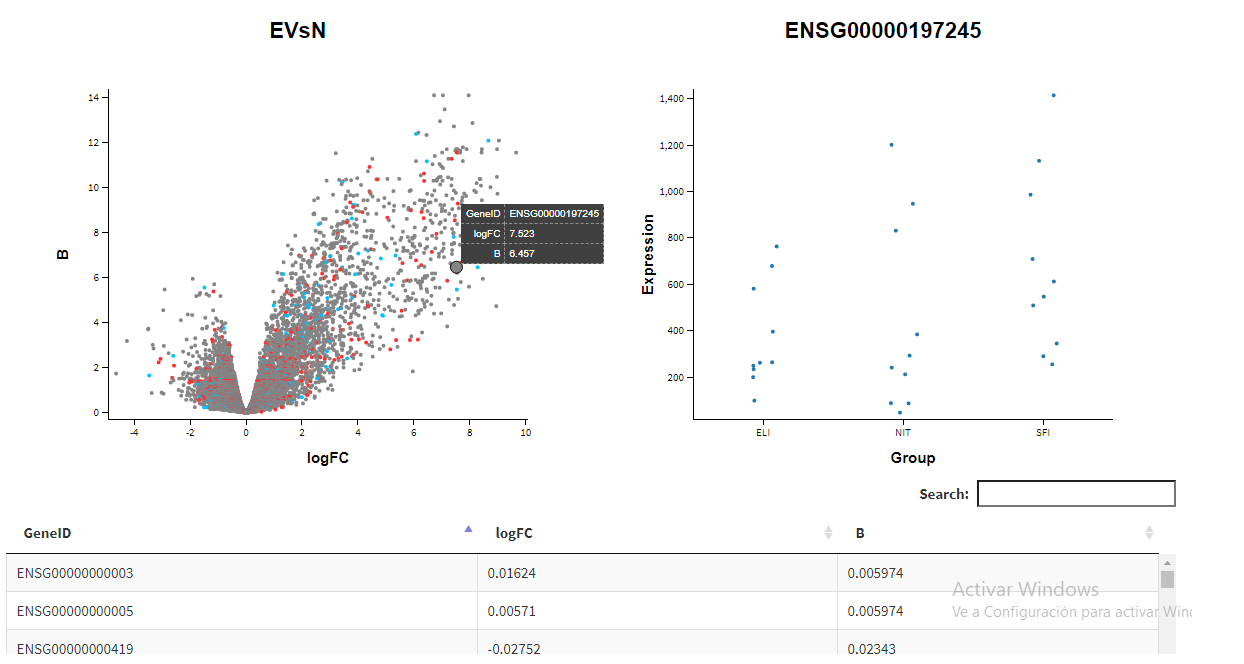
\includegraphics[width=1\linewidth]{C:/Pec2DatosOmicos/results/Glima2} \caption{Diagrama MDS interactivo}\label{fig:unnamed-chunk-46}
\end{figure}

Se podrian hacer más cosas, como recuperar las ubicaciones genomicas,
manipular los intervalos genomicos con GenomicRangers, exportar pistas o
extraer lecturas.

\hypertarget{significaciuxf3n-biologica}{%
\paragraph{Significación biologica}\label{significaciuxf3n-biologica}}

GOseq es un método para realizar análisis de ontología génica (GO)
adecuado para datos de RNA-seq, ya que explica el sesgo de la longitud
del gen en la detección de sobrerepresentación.

\begin{Shaded}
\begin{Highlighting}[]
\CommentTok{# lista de DEGs filtrando con FDR}
\NormalTok{genes <-}\StringTok{ }\NormalTok{results}\OperatorTok{$}\NormalTok{FDR }\OperatorTok{<}\StringTok{ }\FloatTok{0.05}



\CommentTok{# Añadimos nombres}
\KeywordTok{names}\NormalTok{(genes) <-}\StringTok{ }\KeywordTok{rownames}\NormalTok{(results)}
\KeywordTok{print}\NormalTok{(}\KeywordTok{head}\NormalTok{(genes))}
\end{Highlighting}
\end{Shaded}

\begin{verbatim}
## ENSG00000083454 ENSG00000105369 ENSG00000143297 ENSG00000136573 ENSG00000035720 
##            TRUE            TRUE            TRUE            TRUE            TRUE 
## ENSG00000132704 
##            TRUE
\end{verbatim}

Calcularemos una función de ponderación de probabilidad o PWF que puede
considerarse como una función que da la probabilidad de que un gen se
exprese diferencialmente (DE), basándose solo en su longitud.

\begin{Shaded}
\begin{Highlighting}[]
\KeywordTok{supportedOrganisms}\NormalTok{()[}\KeywordTok{supportedOrganisms}\NormalTok{()}\OperatorTok{$}\NormalTok{Genome}\OperatorTok{==}\StringTok{"hg19"}\NormalTok{,]}
\end{Highlighting}
\end{Shaded}

\begin{verbatim}
## Loading required package: rtracklayer
\end{verbatim}

\begin{verbatim}
##    Genome         Id  Id Description Lengths in geneLeneDataBase
## 4    hg19  knownGene  Entrez Gene ID                        TRUE
## 36   hg19    ensGene Ensembl gene ID                        TRUE
## 81   hg19 geneSymbol     Gene Symbol                        TRUE
##    GO Annotation Available
## 4                     TRUE
## 36                    TRUE
## 81                    TRUE
\end{verbatim}

\begin{Shaded}
\begin{Highlighting}[]
\NormalTok{pwf <-}\StringTok{ }\KeywordTok{nullp}\NormalTok{(genes, }\StringTok{"hg19"}\NormalTok{, }\StringTok{"ensGene"}\NormalTok{)}
\end{Highlighting}
\end{Shaded}

\begin{verbatim}
## Loading hg19 length data...
\end{verbatim}

\includegraphics{RuizMacias_EvaM_PEC2_ADO_files/figure-latex/unnamed-chunk-50-1.pdf}

\begin{Shaded}
\begin{Highlighting}[]
\KeywordTok{head}\NormalTok{(pwf)}
\end{Highlighting}
\end{Shaded}

\begin{verbatim}
##                 DEgenes bias.data       pwf
## ENSG00000083454    TRUE    1520.0 0.1353301
## ENSG00000105369    TRUE    1206.0 0.1411115
## ENSG00000143297    TRUE    2196.5 0.1324122
## ENSG00000136573    TRUE    2483.5 0.1324118
## ENSG00000035720    TRUE    1338.0 0.1381760
## ENSG00000132704    TRUE    2591.0 0.1324118
\end{verbatim}

\begin{verbatim}
## Loading hg19 length data...
\end{verbatim}

\begin{verbatim}
## Warning in pcls(G): initial point very close to some inequality constraints
\end{verbatim}

\includegraphics{RuizMacias_EvaM_PEC2_ADO_files/figure-latex/unnamed-chunk-51-1.pdf}

\begin{verbatim}
## Loading hg19 length data...
\end{verbatim}

\includegraphics{RuizMacias_EvaM_PEC2_ADO_files/figure-latex/unnamed-chunk-52-1.pdf}

\begin{Shaded}
\begin{Highlighting}[]
\KeywordTok{write.csv}\NormalTok{(results.annotated,}\DataTypeTok{file=}\StringTok{"C:/Pec2DatosOmicos/results/pwf.tsv"}\NormalTok{,}
          \DataTypeTok{row.names=}\OtherTok{FALSE}\NormalTok{)}
\end{Highlighting}
\end{Shaded}

Las gráficas salen diferente a todas las que he visto en diferentes
documentos, no se si es debido a algun fallo en el analisis, o que el
ajuste es malo.

He probado a hacerlo de esta otra forma, y se obtiene el mismo
resultado:

\begin{Shaded}
\begin{Highlighting}[]
\NormalTok{geness =}\KeywordTok{as.integer}\NormalTok{(}\KeywordTok{p.adjust}\NormalTok{(et12}\OperatorTok{$}\NormalTok{table}\OperatorTok{$}\NormalTok{PValue[et12}\OperatorTok{$}\NormalTok{table}\OperatorTok{$}\NormalTok{logFC}\OperatorTok{!=}\DecValTok{0}\NormalTok{],}
                               \DataTypeTok{method=}\StringTok{"BH"}\NormalTok{)}\OperatorTok{<}\NormalTok{.}\DecValTok{05}\NormalTok{)}
                               \KeywordTok{names}\NormalTok{(geness)=}\KeywordTok{row.names}\NormalTok{(et12}\OperatorTok{$}\NormalTok{table[et12}\OperatorTok{$}\NormalTok{table}\OperatorTok{$}\NormalTok{logFC}\OperatorTok{!=}\DecValTok{0}\NormalTok{,])}
\NormalTok{pwff <-}\StringTok{ }\KeywordTok{nullp}\NormalTok{(geness, }\StringTok{"hg19"}\NormalTok{, }\StringTok{"ensGene"}\NormalTok{)                               }
\end{Highlighting}
\end{Shaded}

Realizamos un análisis de enriquecimiento del conjunto de genes:

\begin{Shaded}
\begin{Highlighting}[]
\NormalTok{go.results <-}\StringTok{ }\KeywordTok{goseq}\NormalTok{(pwf, }\StringTok{"hg19"}\NormalTok{, }\StringTok{"ensGene"}\NormalTok{)}
\end{Highlighting}
\end{Shaded}

\begin{verbatim}
## Fetching GO annotations...
\end{verbatim}

\begin{verbatim}
## For 6343 genes, we could not find any categories. These genes will be excluded.
\end{verbatim}

\begin{verbatim}
## To force their use, please run with use_genes_without_cat=TRUE (see documentation).
\end{verbatim}

\begin{verbatim}
## This was the default behavior for version 1.15.1 and earlier.
\end{verbatim}

\begin{verbatim}
## Calculating the p-values...
\end{verbatim}

\begin{verbatim}
## 'select()' returned 1:1 mapping between keys and columns
\end{verbatim}

\begin{Shaded}
\begin{Highlighting}[]
\KeywordTok{head}\NormalTok{(go.results)}
\end{Highlighting}
\end{Shaded}

\begin{verbatim}
##         category over_represented_pvalue under_represented_pvalue numDEInCat
## 1024  GO:0002376            1.127899e-58                        1        621
## 2816  GO:0005886            4.298089e-53                        1        875
## 16713 GO:0071944            1.006569e-52                        1        891
## 3517  GO:0006955            5.775350e-51                        1        458
## 12622 GO:0046649            1.705570e-48                        1        220
## 938   GO:0002250            8.795023e-48                        1        162
##       numInCat                     term ontology
## 1024      2582    immune system process       BP
## 2816      4298          plasma membrane       CC
## 16713     4410           cell periphery       CC
## 3517      1762          immune response       BP
## 12622      604    lymphocyte activation       BP
## 938        370 adaptive immune response       BP
\end{verbatim}

\begin{Shaded}
\begin{Highlighting}[]
\NormalTok{enriched.GO=go.results}\OperatorTok{$}\NormalTok{category[}\KeywordTok{p.adjust}\NormalTok{(go.results}\OperatorTok{$}\NormalTok{over_represented_pvalue,}
                                      \DataTypeTok{method=}\StringTok{"BH"}\NormalTok{)}\OperatorTok{<}\NormalTok{.}\DecValTok{05}\NormalTok{]}

\KeywordTok{head}\NormalTok{(enriched.GO)}
\end{Highlighting}
\end{Shaded}

\begin{verbatim}
## [1] "GO:0002376" "GO:0005886" "GO:0071944" "GO:0006955" "GO:0046649"
## [6] "GO:0002250"
\end{verbatim}

Categorías GO relacionadas:

\begin{Shaded}
\begin{Highlighting}[]
\ControlFlowTok{for}\NormalTok{(go }\ControlFlowTok{in}\NormalTok{ enriched.GO[}\DecValTok{1}\OperatorTok{:}\DecValTok{5}\NormalTok{])\{}
  \KeywordTok{print}\NormalTok{(GOTERM[[go]])}
  \KeywordTok{cat}\NormalTok{(}\StringTok{"--------------------------------------}\CharTok{\textbackslash{}n}\StringTok{"}\NormalTok{)}
\NormalTok{  \}}
\end{Highlighting}
\end{Shaded}

\begin{verbatim}
## GOID: GO:0002376
## Term: immune system process
## Ontology: BP
## Definition: Any process involved in the development or functioning of
##     the immune system, an organismal system for calibrated responses to
##     potential internal or invasive threats.
## --------------------------------------
## GOID: GO:0005886
## Term: plasma membrane
## Ontology: CC
## Definition: The membrane surrounding a cell that separates the cell
##     from its external environment. It consists of a phospholipid
##     bilayer and associated proteins.
## Synonym: bacterial inner membrane
## Synonym: cell membrane
## Synonym: cellular membrane
## Synonym: cytoplasmic membrane
## Synonym: inner endospore membrane
## Synonym: juxtamembrane
## Synonym: plasma membrane lipid bilayer
## Synonym: plasmalemma
## Synonym: GO:0005904
## Secondary: GO:0005904
## --------------------------------------
## GOID: GO:0071944
## Term: cell periphery
## Ontology: CC
## Definition: The part of a cell encompassing the cell cortex, the plasma
##     membrane, and any external encapsulating structures.
## --------------------------------------
## GOID: GO:0006955
## Term: immune response
## Ontology: BP
## Definition: Any immune system process that functions in the calibrated
##     response of an organism to a potential internal or invasive threat.
## --------------------------------------
## GOID: GO:0046649
## Term: lymphocyte activation
## Ontology: BP
## Definition: A change in morphology and behavior of a lymphocyte
##     resulting from exposure to a specific antigen, mitogen, cytokine,
##     chemokine, cellular ligand, or soluble factor.
## --------------------------------------
\end{verbatim}

También podriamos haber hecho el analisis de significación biologica con
la herramienta en linea Enrich, para lo cual necesitariamos subir a la
plataforma de Enrich el archivo con las anotaciones de los genes.

El paquete fgsea que aleatoriza reiteradamente las etiquetas de las
muestras y vuelve a realizar pruebas de enriquecimiento en las clases
aleatorias.

\hypertarget{resultados}{%
\section{Resultados}\label{resultados}}

Aqui se mostrara una lista de archivos generados en el estudio de caso
actual.

\begin{Shaded}
\begin{Highlighting}[]
\NormalTok{listOfFiles <-}\StringTok{ }\KeywordTok{dir}\NormalTok{(}\StringTok{"./results/"}\NormalTok{) }
\NormalTok{knitr}\OperatorTok{::}\KeywordTok{kable}\NormalTok{(}
\NormalTok{  listOfFiles, }\DataTypeTok{booktabs =} \OtherTok{TRUE}\NormalTok{,}
  \DataTypeTok{caption =} \StringTok{'List of files generated in the analysis'}\NormalTok{,}
  \DataTypeTok{col.names=}\StringTok{"List_of_Files"}
\NormalTok{)}
\end{Highlighting}
\end{Shaded}

\begin{table}

\caption{\label{tab:unnamed-chunk-58}List of files generated in the analysis}
\centering
\begin{tabular}[t]{l}
\toprule
List\_of\_Files\\
\midrule
DE.Rdata\\
ELIVsNIT.csv\\
ELIVsSFI.csv\\
Glima1.png\\
Glima2.png\\
\addlinespace
NITVsSFI.csv\\
preprocessing.Rdata\\
pwf.tsv\\
pwf2.tsv\\
pwf3.tsv\\
\bottomrule
\end{tabular}
\end{table}

\hypertarget{apendice}{%
\section{Apendice}\label{apendice}}

\hypertarget{anotaciuxf3n-y-visualizaciuxf3n-de-resultados-1}{%
\subsection{Anotación y visualización de
resultados}\label{anotaciuxf3n-y-visualizaciuxf3n-de-resultados-1}}

\begin{Shaded}
\begin{Highlighting}[]
\NormalTok{ann2 <-}\StringTok{ }\KeywordTok{select}\NormalTok{(org.Hs.eg.db,}\DataTypeTok{keys=}\KeywordTok{rownames}\NormalTok{(results2), }\DataTypeTok{keytype =} \StringTok{"ENSEMBL"}\NormalTok{,}
              \DataTypeTok{columns=}\KeywordTok{c}\NormalTok{(}\StringTok{"SYMBOL"}\NormalTok{,}\StringTok{"GENENAME"}\NormalTok{))}
\NormalTok{ann3 <-}\StringTok{ }\KeywordTok{select}\NormalTok{(org.Hs.eg.db,}\DataTypeTok{keys=}\KeywordTok{rownames}\NormalTok{(results3), }\DataTypeTok{keytype =} \StringTok{"ENSEMBL"}\NormalTok{,}
              \DataTypeTok{columns=}\KeywordTok{c}\NormalTok{(}\StringTok{"SYMBOL"}\NormalTok{,}\StringTok{"GENENAME"}\NormalTok{))}
\end{Highlighting}
\end{Shaded}

Verifiquemos nuevamente que la columna ENSEMBL coincida exactamente con
los nombres de las filas de results.

\begin{Shaded}
\begin{Highlighting}[]
\CommentTok{# Tengo que hacer esto debido a la salida 'select()' returned 1:many...}
\NormalTok{ann2 <-}\StringTok{ }\NormalTok{ann2[}\OperatorTok{!}\KeywordTok{duplicated}\NormalTok{(ann2}\OperatorTok{$}\NormalTok{ENSEMBL), ] }
\NormalTok{results.annotated2 <-}\StringTok{ }\KeywordTok{cbind}\NormalTok{(results2, ann2)}



\NormalTok{ann3 <-}\StringTok{ }\NormalTok{ann3[}\OperatorTok{!}\KeywordTok{duplicated}\NormalTok{(ann3}\OperatorTok{$}\NormalTok{ENSEMBL), ] }
\NormalTok{results.annotated3 <-}\StringTok{ }\KeywordTok{cbind}\NormalTok{(results3, ann3)}
\end{Highlighting}
\end{Shaded}

\begin{Shaded}
\begin{Highlighting}[]
\NormalTok{detags <-}\StringTok{ }\KeywordTok{rownames}\NormalTok{(dgList)[}\KeywordTok{as.logical}\NormalTok{(de2es)]}
\NormalTok{signif <-}\StringTok{ }\OperatorTok{-}\KeywordTok{log10}\NormalTok{(results.annotated}\OperatorTok{$}\NormalTok{FDR)}
\KeywordTok{plot}\NormalTok{(results.annotated}\OperatorTok{$}\NormalTok{logFC,signif,}\DataTypeTok{pch=}\DecValTok{16}\NormalTok{)}
\KeywordTok{points}\NormalTok{(results.annotated[detags,}\StringTok{"logFC"}\NormalTok{],}\OperatorTok{-}\KeywordTok{log10}\NormalTok{(results.annotated[detags,}\StringTok{"FDR"}\NormalTok{]),}\DataTypeTok{pch=}\DecValTok{16}\NormalTok{,}\DataTypeTok{col=}\StringTok{"red"}\NormalTok{)}

\CommentTok{#ggplot(results, aes(x = logFC, y=-log10(FDR))) + geom_point()}

\NormalTok{detags <-}\StringTok{ }\KeywordTok{rownames}\NormalTok{(dgList)[}\KeywordTok{as.logical}\NormalTok{(de2ns)]}
\NormalTok{signif <-}\StringTok{ }\OperatorTok{-}\KeywordTok{log10}\NormalTok{(results.annotated}\OperatorTok{$}\NormalTok{FDR)}
\KeywordTok{plot}\NormalTok{(results.annotated}\OperatorTok{$}\NormalTok{logFC,signif,}\DataTypeTok{pch=}\DecValTok{16}\NormalTok{)}
\KeywordTok{points}\NormalTok{(results.annotated[detags,}\StringTok{"logFC"}\NormalTok{],}\OperatorTok{-}\KeywordTok{log10}\NormalTok{(results.annotated[detags,}\StringTok{"FDR"}\NormalTok{]),}\DataTypeTok{pch=}\DecValTok{16}\NormalTok{,}\DataTypeTok{col=}\StringTok{"red"}\NormalTok{)}

\CommentTok{#ggplot(results, aes(x = logFC, y=-log10(FDR))) + geom_point()}
\end{Highlighting}
\end{Shaded}

\hypertarget{significaciuxf3n-biologica-1}{%
\subsection{Significación
biologica}\label{significaciuxf3n-biologica-1}}

\begin{Shaded}
\begin{Highlighting}[]
\CommentTok{# lista de DEGs filtrando con FDR}
\NormalTok{genes2 <-}\StringTok{ }\NormalTok{results2}\OperatorTok{$}\NormalTok{FDR }\OperatorTok{<}\StringTok{ }\FloatTok{0.01}

\CommentTok{# Añadimos nombres}
\KeywordTok{names}\NormalTok{(genes2) <-}\StringTok{ }\KeywordTok{rownames}\NormalTok{(results2)}

\KeywordTok{print}\NormalTok{(}\KeywordTok{head}\NormalTok{(genes2))}
\end{Highlighting}
\end{Shaded}

\begin{Shaded}
\begin{Highlighting}[]
\CommentTok{# lista de DEGs filtrando con FDR}
\NormalTok{genes3 <-}\StringTok{ }\NormalTok{results3}\OperatorTok{$}\NormalTok{FDR }\OperatorTok{<}\StringTok{ }\FloatTok{0.01}

\CommentTok{# Añadimos nombres}
\KeywordTok{names}\NormalTok{(genes3) <-}\StringTok{ }\KeywordTok{rownames}\NormalTok{(results3)}

\KeywordTok{print}\NormalTok{(}\KeywordTok{head}\NormalTok{(genes3))}
\end{Highlighting}
\end{Shaded}

\begin{Shaded}
\begin{Highlighting}[]
\NormalTok{pwf2 <-}\StringTok{ }\KeywordTok{nullp}\NormalTok{(genes2, }\StringTok{"hg19"}\NormalTok{, }\StringTok{"ensGene"}\NormalTok{)}
\KeywordTok{head}\NormalTok{(pwf2)}
\end{Highlighting}
\end{Shaded}

\begin{Shaded}
\begin{Highlighting}[]
\NormalTok{pwf3 <-}\StringTok{ }\KeywordTok{nullp}\NormalTok{(genes3, }\StringTok{"hg19"}\NormalTok{, }\StringTok{"ensGene"}\NormalTok{)}
\KeywordTok{head}\NormalTok{(pwf3)}
\end{Highlighting}
\end{Shaded}

\begin{Shaded}
\begin{Highlighting}[]
\KeywordTok{write.csv}\NormalTok{(results.annotated,}\DataTypeTok{file=}\StringTok{"C:/Pec2DatosOmicos/results/pwf2.tsv"}\NormalTok{,}
          \DataTypeTok{row.names=}\OtherTok{FALSE}\NormalTok{)}
\KeywordTok{write.csv}\NormalTok{(results.annotated,}\DataTypeTok{file=}\StringTok{"C:/Pec2DatosOmicos/results/pwf3.tsv"}\NormalTok{,}
          \DataTypeTok{row.names=}\OtherTok{FALSE}\NormalTok{)}
\end{Highlighting}
\end{Shaded}

\begin{Shaded}
\begin{Highlighting}[]
\NormalTok{go.results2 <-}\StringTok{ }\KeywordTok{goseq}\NormalTok{(pwf2, }\StringTok{"hg19"}\NormalTok{, }\StringTok{"ensGene"}\NormalTok{)}
\end{Highlighting}
\end{Shaded}

\begin{verbatim}
## Fetching GO annotations...
\end{verbatim}

\begin{verbatim}
## For 6343 genes, we could not find any categories. These genes will be excluded.
\end{verbatim}

\begin{verbatim}
## To force their use, please run with use_genes_without_cat=TRUE (see documentation).
\end{verbatim}

\begin{verbatim}
## This was the default behavior for version 1.15.1 and earlier.
\end{verbatim}

\begin{verbatim}
## Calculating the p-values...
\end{verbatim}

\begin{verbatim}
## 'select()' returned 1:1 mapping between keys and columns
\end{verbatim}

\begin{Shaded}
\begin{Highlighting}[]
\KeywordTok{head}\NormalTok{(go.results2)}
\end{Highlighting}
\end{Shaded}

\begin{verbatim}
##         category over_represented_pvalue under_represented_pvalue numDEInCat
## 2654  GO:0005615            1.215104e-07                1.0000000         72
## 11674 GO:0044421            3.199790e-07                1.0000000         74
## 13314 GO:0048870            3.309123e-07                0.9999999         47
## 14060 GO:0051674            3.309123e-07                0.9999999         47
## 5874  GO:0016477            4.173663e-07                0.9999999         44
## 7535  GO:0030855            4.203663e-07                0.9999999         26
##       numInCat                            term ontology
## 2654      2703             extracellular space       CC
## 11674     2872       extracellular region part       CC
## 13314     1412                   cell motility       BP
## 14060     1412            localization of cell       BP
## 5874      1283                  cell migration       BP
## 7535       551 epithelial cell differentiation       BP
\end{verbatim}

\begin{Shaded}
\begin{Highlighting}[]
\NormalTok{enriched.GO2=go.results2}\OperatorTok{$}\NormalTok{category[}\KeywordTok{p.adjust}\NormalTok{(go.results2}\OperatorTok{$}\NormalTok{over_represented_pvalue,}
                                      \DataTypeTok{method=}\StringTok{"BH"}\NormalTok{)}\OperatorTok{<}\NormalTok{.}\DecValTok{05}\NormalTok{]}

\KeywordTok{head}\NormalTok{(enriched.GO2)}
\end{Highlighting}
\end{Shaded}

\begin{verbatim}
## [1] "GO:0005615" "GO:0044421" "GO:0048870" "GO:0051674" "GO:0016477"
## [6] "GO:0030855"
\end{verbatim}

Categorías GO relacionadas:

\begin{Shaded}
\begin{Highlighting}[]
\ControlFlowTok{for}\NormalTok{(go }\ControlFlowTok{in}\NormalTok{ enriched.GO2[}\DecValTok{1}\OperatorTok{:}\DecValTok{5}\NormalTok{])\{}
  \KeywordTok{print}\NormalTok{(GOTERM[[go]])}
  \KeywordTok{cat}\NormalTok{(}\StringTok{"--------------------------------------}\CharTok{\textbackslash{}n}\StringTok{"}\NormalTok{)}
\NormalTok{  \}}
\end{Highlighting}
\end{Shaded}

\begin{verbatim}
## GOID: GO:0005615
## Term: extracellular space
## Ontology: CC
## Definition: That part of a multicellular organism outside the cells
##     proper, usually taken to be outside the plasma membranes, and
##     occupied by fluid.
## Synonym: intercellular space
## --------------------------------------
## GOID: GO:0044421
## Term: extracellular region part
## Ontology: CC
## Definition: Any constituent part of the extracellular region, the space
##     external to the outermost structure of a cell. For cells without
##     external protective or external encapsulating structures this
##     refers to space outside of the plasma membrane. This term covers
##     constituent parts of the host cell environment outside an
##     intracellular parasite.
## Synonym: extracellular structure
## --------------------------------------
## GOID: GO:0048870
## Term: cell motility
## Ontology: BP
## Definition: Any process involved in the controlled self-propelled
##     movement of a cell that results in translocation of the cell from
##     one place to another.
## Synonym: cell locomotion
## Synonym: cell movement
## Synonym: movement of a cell
## --------------------------------------
## GOID: GO:0051674
## Term: localization of cell
## Ontology: BP
## Definition: Any process in which a cell is transported to, and/or
##     maintained in, a specific location.
## Synonym: cell localization
## Synonym: establishment and maintenance of cell localization
## Synonym: establishment and maintenance of localization of cell
## Synonym: localisation of cell
## --------------------------------------
## GOID: GO:0016477
## Term: cell migration
## Ontology: BP
## Definition: The controlled self-propelled movement of a cell from one
##     site to a destination guided by molecular cues. Cell migration is a
##     central process in the development and maintenance of multicellular
##     organisms.
## --------------------------------------
\end{verbatim}

\begin{Shaded}
\begin{Highlighting}[]
\NormalTok{go.results3 <-}\StringTok{ }\KeywordTok{goseq}\NormalTok{(pwf3, }\StringTok{"hg19"}\NormalTok{, }\StringTok{"ensGene"}\NormalTok{)}
\end{Highlighting}
\end{Shaded}

\begin{verbatim}
## Fetching GO annotations...
\end{verbatim}

\begin{verbatim}
## For 6343 genes, we could not find any categories. These genes will be excluded.
\end{verbatim}

\begin{verbatim}
## To force their use, please run with use_genes_without_cat=TRUE (see documentation).
\end{verbatim}

\begin{verbatim}
## This was the default behavior for version 1.15.1 and earlier.
\end{verbatim}

\begin{verbatim}
## Calculating the p-values...
\end{verbatim}

\begin{verbatim}
## 'select()' returned 1:1 mapping between keys and columns
\end{verbatim}

\begin{Shaded}
\begin{Highlighting}[]
\KeywordTok{head}\NormalTok{(go.results3)}
\end{Highlighting}
\end{Shaded}

\begin{verbatim}
##         category over_represented_pvalue under_represented_pvalue numDEInCat
## 938   GO:0002250            1.601071e-36                        1         44
## 12622 GO:0046649            2.326891e-34                        1         50
## 1024  GO:0002376            1.801146e-32                        1         90
## 3517  GO:0006955            2.100249e-29                        1         74
## 1194  GO:0002682            1.043842e-27                        1         63
## 12003 GO:0045321            8.395021e-26                        1         56
##       numInCat                                term ontology
## 938        370            adaptive immune response       BP
## 12622      604               lymphocyte activation       BP
## 1024      2582               immune system process       BP
## 3517      1762                     immune response       BP
## 1194      1366 regulation of immune system process       BP
## 12003     1124                leukocyte activation       BP
\end{verbatim}

\begin{Shaded}
\begin{Highlighting}[]
\NormalTok{enriched.GO3=go.results3}\OperatorTok{$}\NormalTok{category[}\KeywordTok{p.adjust}\NormalTok{(go.results3}\OperatorTok{$}\NormalTok{over_represented_pvalue,}
                                      \DataTypeTok{method=}\StringTok{"BH"}\NormalTok{)}\OperatorTok{<}\NormalTok{.}\DecValTok{05}\NormalTok{]}

\KeywordTok{head}\NormalTok{(enriched.GO3)}
\end{Highlighting}
\end{Shaded}

\begin{verbatim}
## [1] "GO:0002250" "GO:0046649" "GO:0002376" "GO:0006955" "GO:0002682"
## [6] "GO:0045321"
\end{verbatim}

Categorías GO relacionadas:

\begin{Shaded}
\begin{Highlighting}[]
\ControlFlowTok{for}\NormalTok{(go }\ControlFlowTok{in}\NormalTok{ enriched.GO3[}\DecValTok{1}\OperatorTok{:}\DecValTok{5}\NormalTok{])\{}
  \KeywordTok{print}\NormalTok{(GOTERM[[go]])}
  \KeywordTok{cat}\NormalTok{(}\StringTok{"--------------------------------------}\CharTok{\textbackslash{}n}\StringTok{"}\NormalTok{)}
\NormalTok{  \}}
\end{Highlighting}
\end{Shaded}

\begin{verbatim}
## GOID: GO:0002250
## Term: adaptive immune response
## Ontology: BP
## Definition: An immune response mediated by cells expressing specific
##     receptors for antigen produced through a somatic diversification
##     process, and allowing for an enhanced secondary response to
##     subsequent exposures to the same antigen (immunological memory).
## Synonym: acquired immune response
## Synonym: immune memory response
## --------------------------------------
## GOID: GO:0046649
## Term: lymphocyte activation
## Ontology: BP
## Definition: A change in morphology and behavior of a lymphocyte
##     resulting from exposure to a specific antigen, mitogen, cytokine,
##     chemokine, cellular ligand, or soluble factor.
## --------------------------------------
## GOID: GO:0002376
## Term: immune system process
## Ontology: BP
## Definition: Any process involved in the development or functioning of
##     the immune system, an organismal system for calibrated responses to
##     potential internal or invasive threats.
## --------------------------------------
## GOID: GO:0006955
## Term: immune response
## Ontology: BP
## Definition: Any immune system process that functions in the calibrated
##     response of an organism to a potential internal or invasive threat.
## --------------------------------------
## GOID: GO:0002682
## Term: regulation of immune system process
## Ontology: BP
## Definition: Any process that modulates the frequency, rate, or extent
##     of an immune system process.
## --------------------------------------
\end{verbatim}

\end{document}
